% An appendix
%======================================================================
\chapter{Molecular Orbitals Diagrams} \label{app.mos}
\markright{Molecular Orbitals Diagrams}
%======================================================================

Frontier \glspl{ac.mo} for each compound discussed in this thesis are listed below in \Cref{fig.mo21,fig.mo22,fig.mo23,fig.mo24,fig.mo25,fig.mo26,fig.mo27,fig.mo28}. These orbitals are generated with the Chemissian program\autocite{chemissian}.

\begin{figure}[!ht]
 \centering
 \begin{subfigure}[b]{0.31\textwidth}
  \includegraphics[clip=true, width=\textwidth, keepaspectratio]{images/mos/1l+2.eps}
  \caption{LUMO+2}
 \end{subfigure}
  \begin{subfigure}[b]{0.31\textwidth}
  \includegraphics[clip=true, width=\textwidth, keepaspectratio]{images/mos/1l+1.eps}
  \caption{LUMO+1}
 \end{subfigure}
  \begin{subfigure}[b]{0.31\textwidth}
  \includegraphics[clip=true, width=\textwidth, keepaspectratio]{images/mos/1l.eps}
  \caption{LUMO}
 \end{subfigure}
 \begin{subfigure}[b]{0.31\textwidth}
  \includegraphics[clip=true, width=\textwidth, keepaspectratio]{images/mos/1h.eps}
  \caption{HOMO}
 \end{subfigure}
 \begin{subfigure}[b]{0.31\textwidth}
  \includegraphics[clip=true, width=\textwidth, keepaspectratio]{images/mos/1h-1.eps}
  \caption{HOMO-1}
 \end{subfigure}
 \begin{subfigure}[b]{0.31\textwidth}
  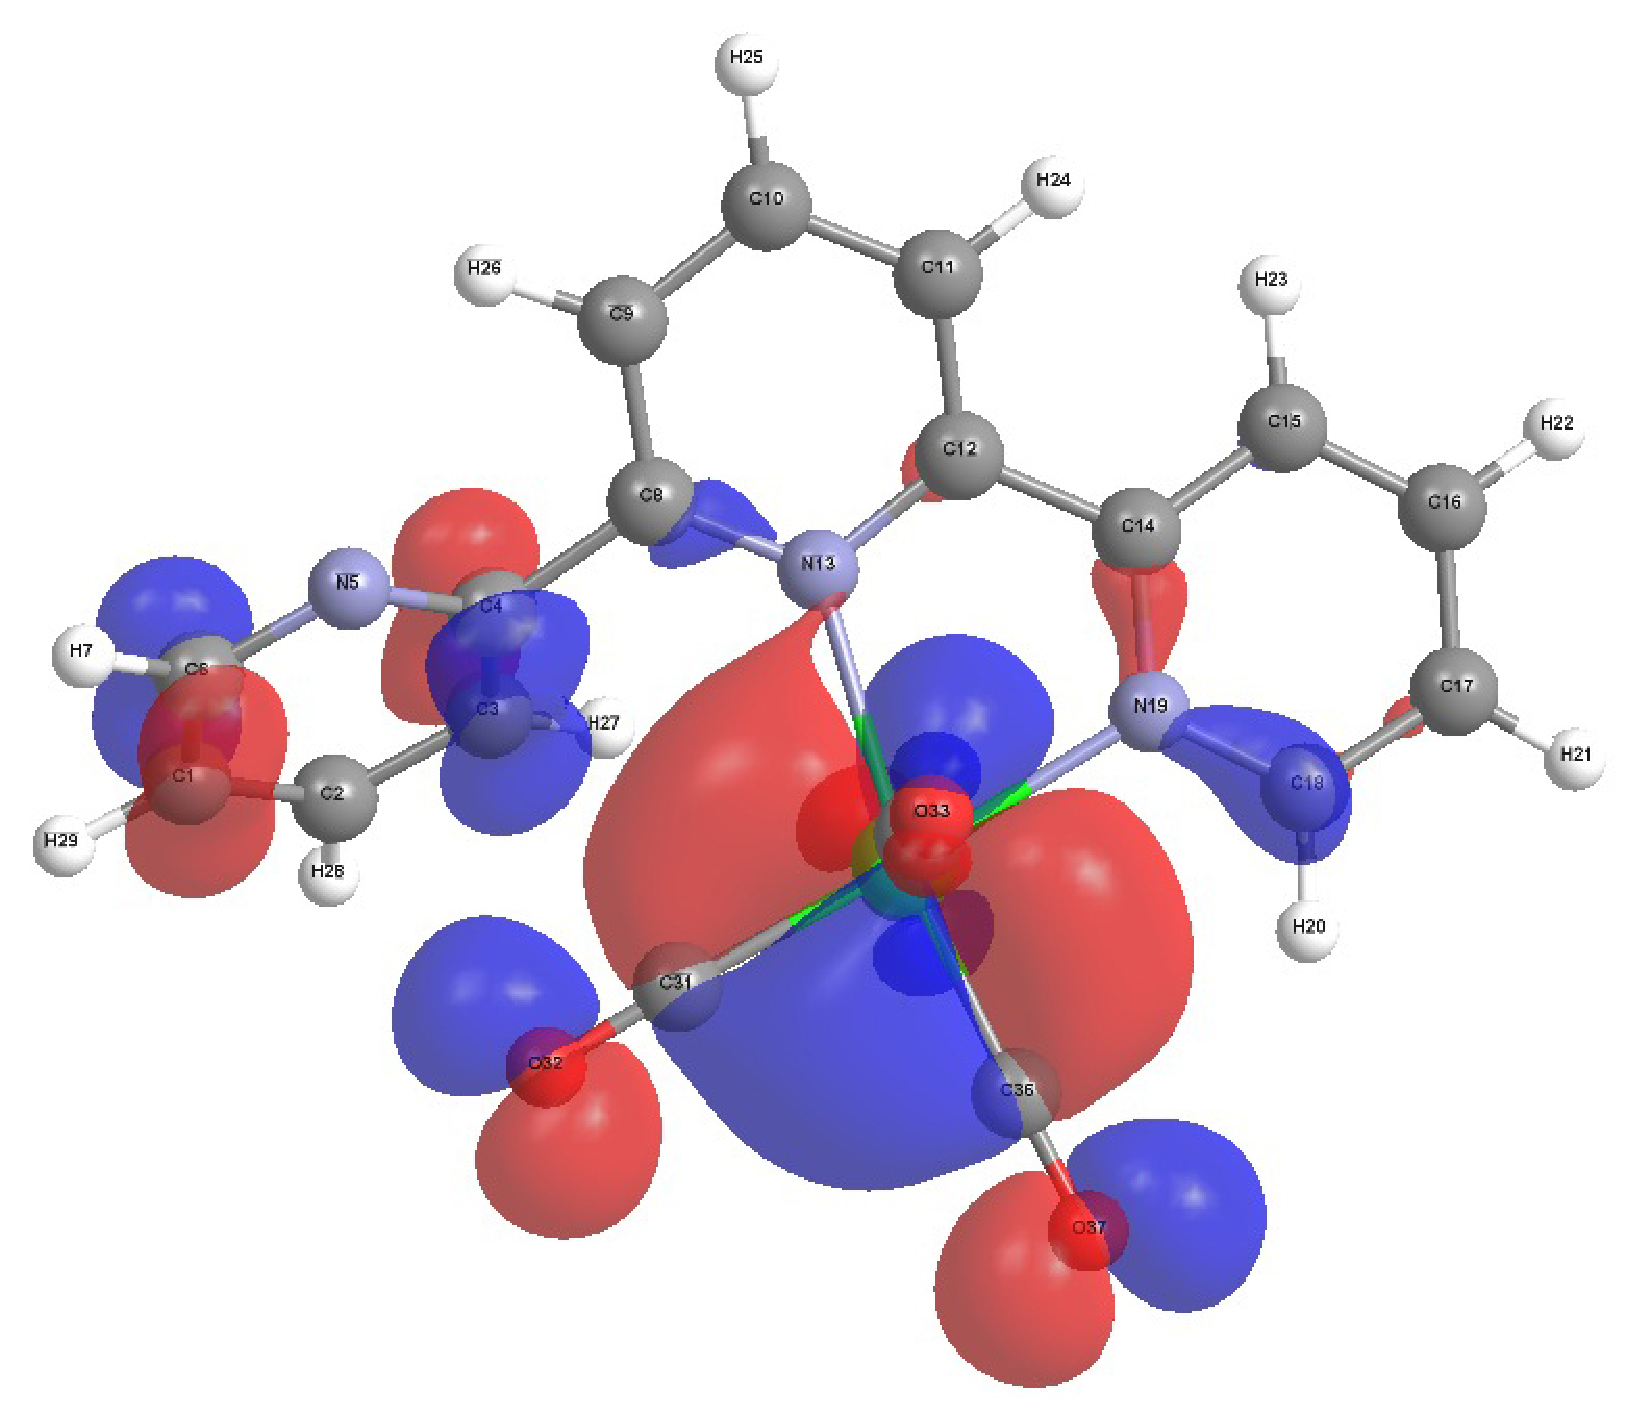
\includegraphics[clip=true, width=\textwidth, keepaspectratio]{images/mos/1h-2.eps}
  \caption{HOMO-2}
 \end{subfigure}
 \begin{subfigure}[b]{0.31\textwidth}
  \includegraphics[clip=true, width=\textwidth, keepaspectratio]{images/mos/1h-3.eps}
  \caption{HOMO-3}
 \end{subfigure}
\caption[Molecular orbitals HOMO-3 to LUMO+2 of \textbf{2.1}]{Isosurface plots of the frontier molecular orbitals HOMO-3 to LUMO+2 of \textbf{2.1}}
\label{fig.mo21}
\end{figure} 

\begin{figure}[!ht]
 \centering
 \begin{subfigure}[b]{0.31\textwidth}
  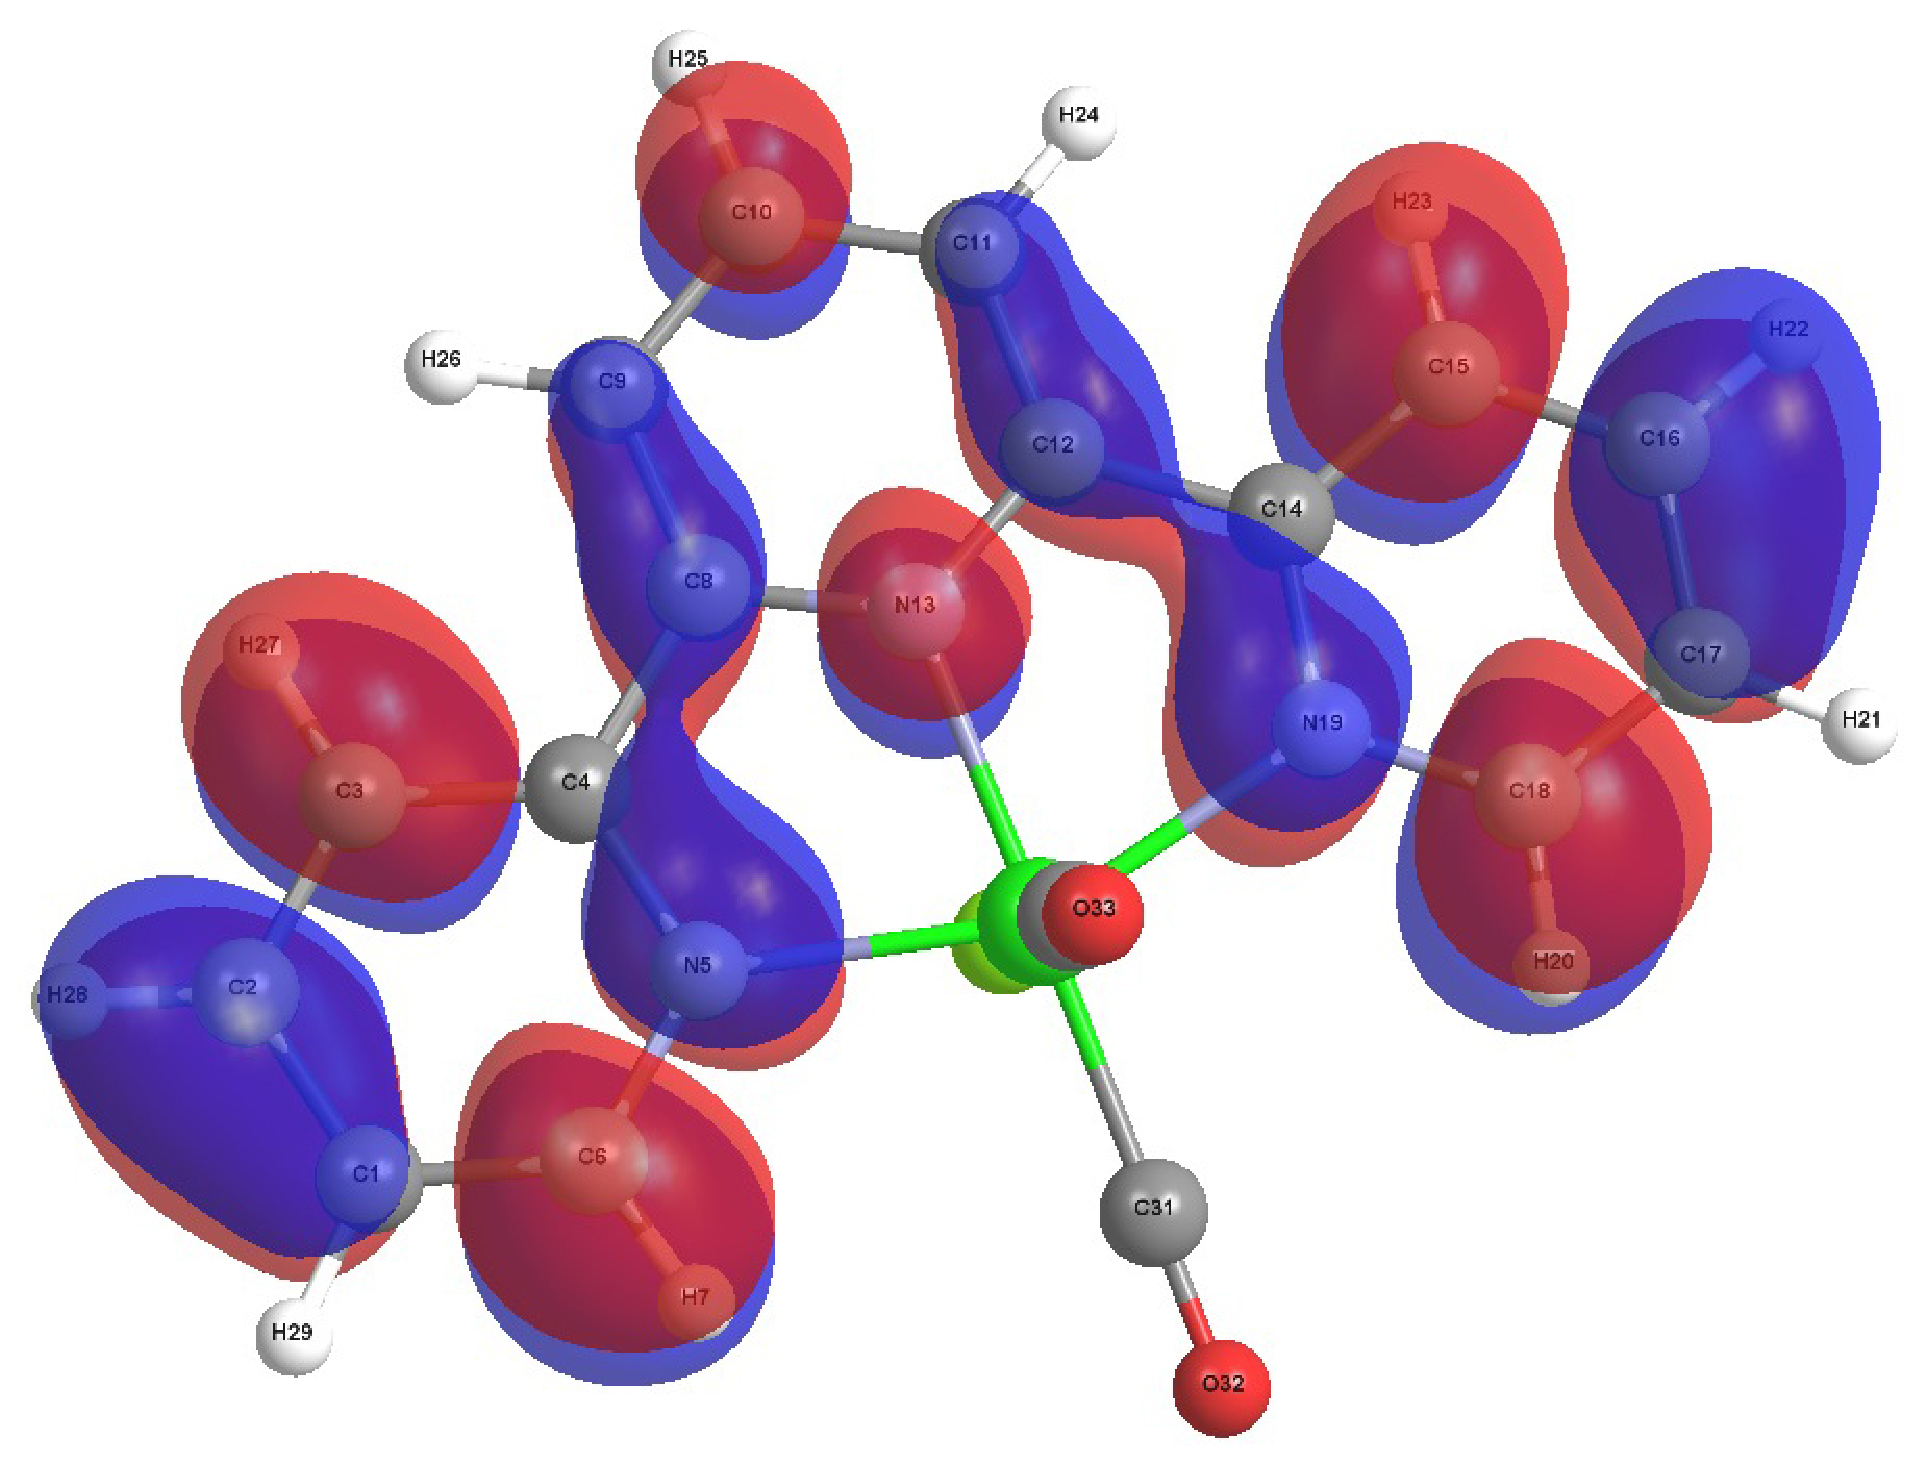
\includegraphics[clip=true, width=\textwidth, keepaspectratio]{images/mos/2l+3.eps}
  \caption{LUMO+3}
 \end{subfigure}
 \begin{subfigure}[b]{0.31\textwidth}
  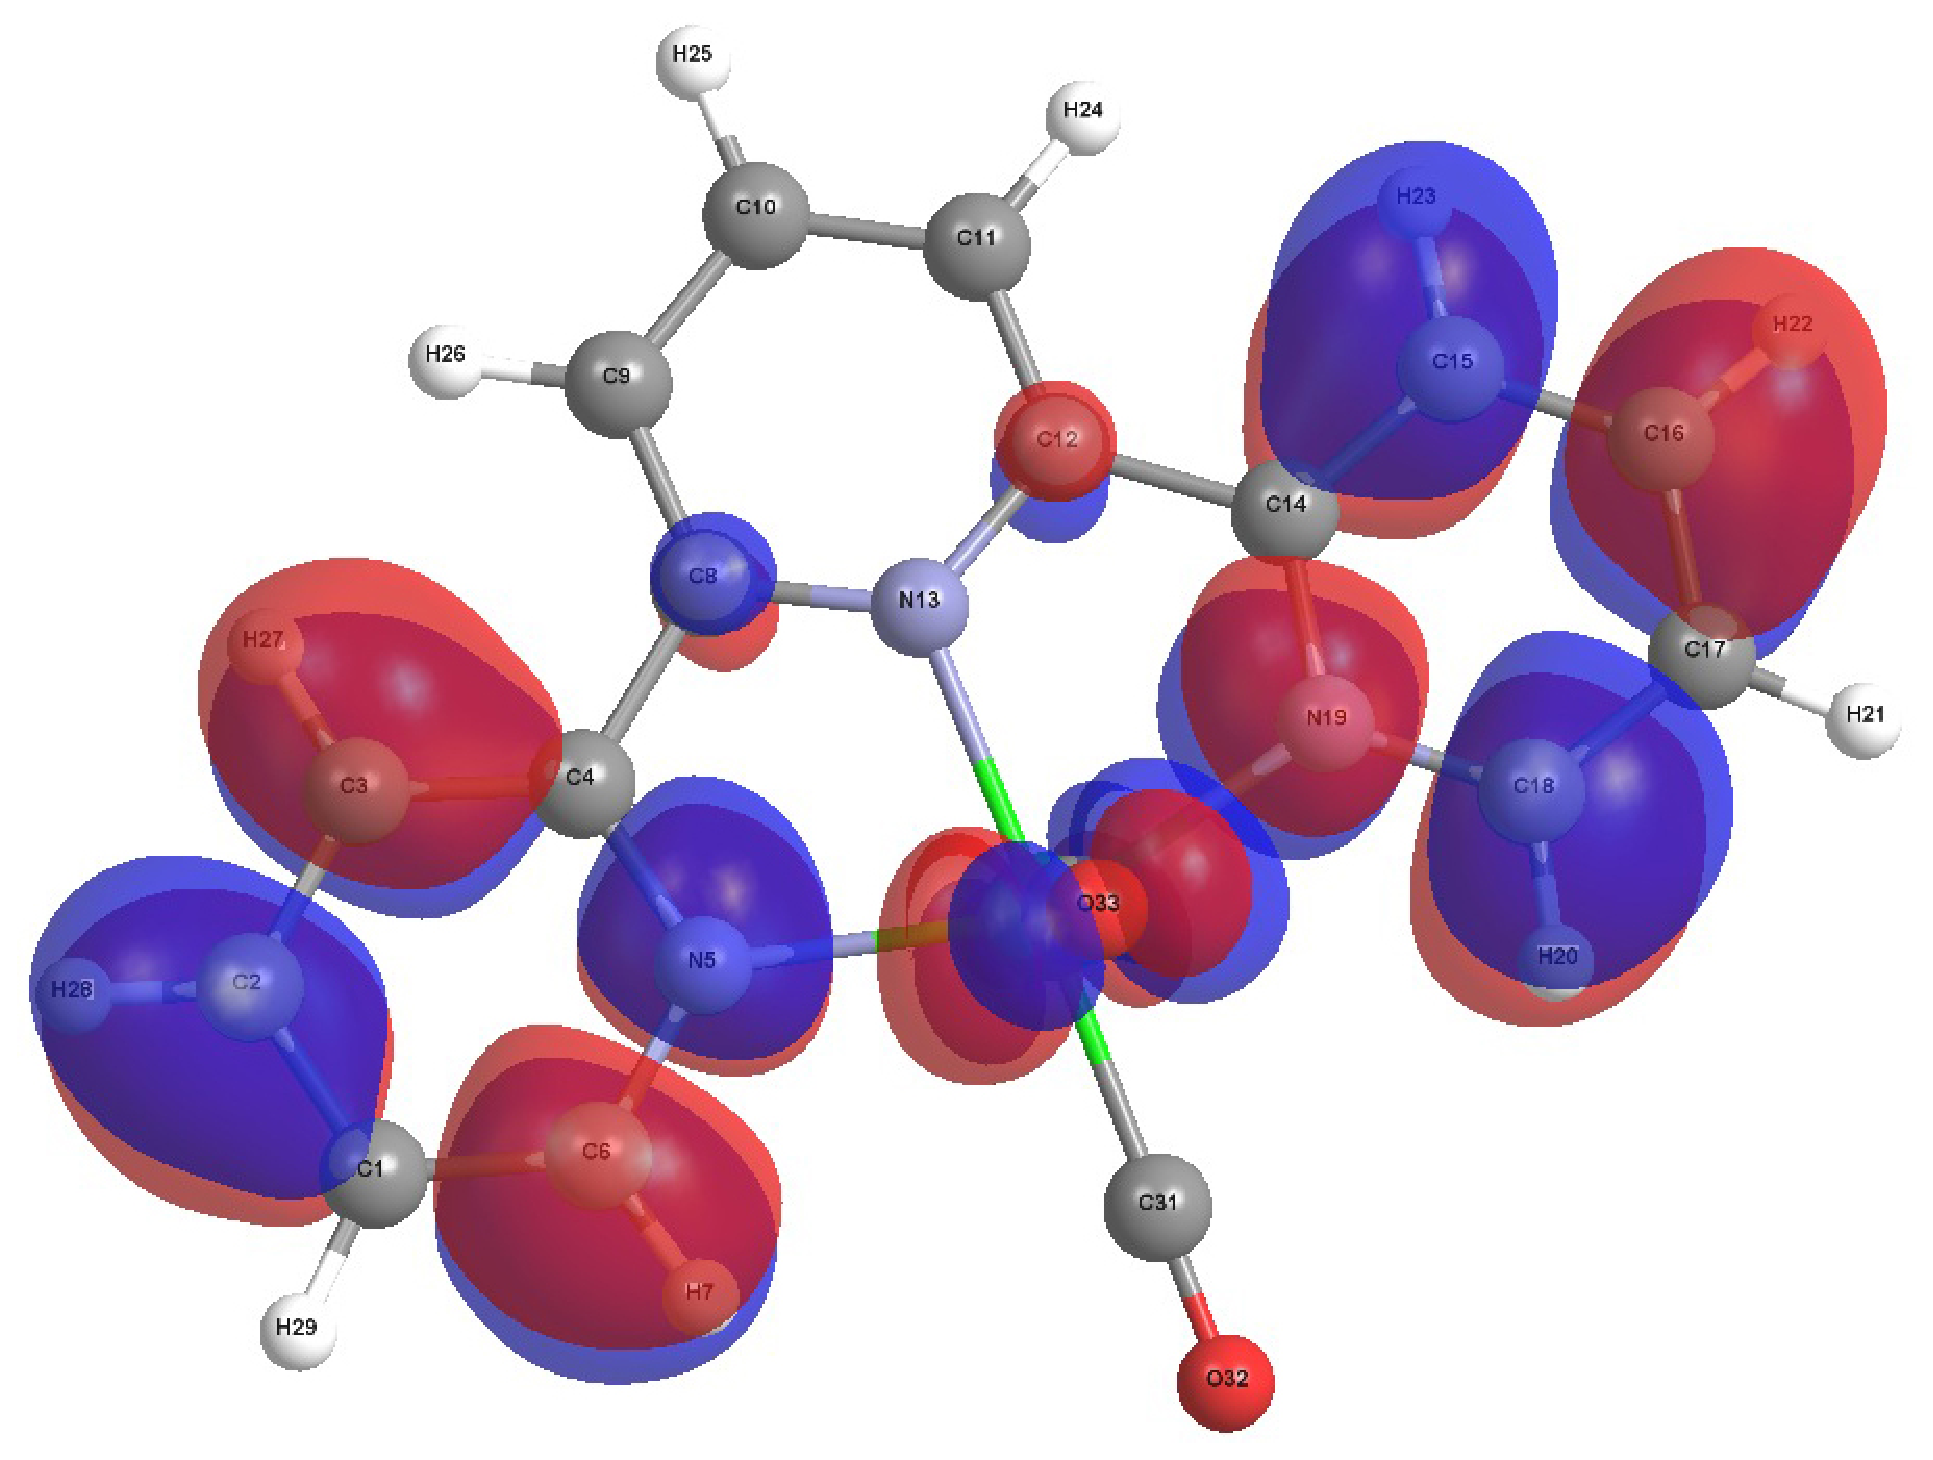
\includegraphics[clip=true, width=\textwidth, keepaspectratio]{images/mos/2l+2.eps}
  \caption{LUMO+2}
 \end{subfigure}
  \begin{subfigure}[b]{0.31\textwidth}
  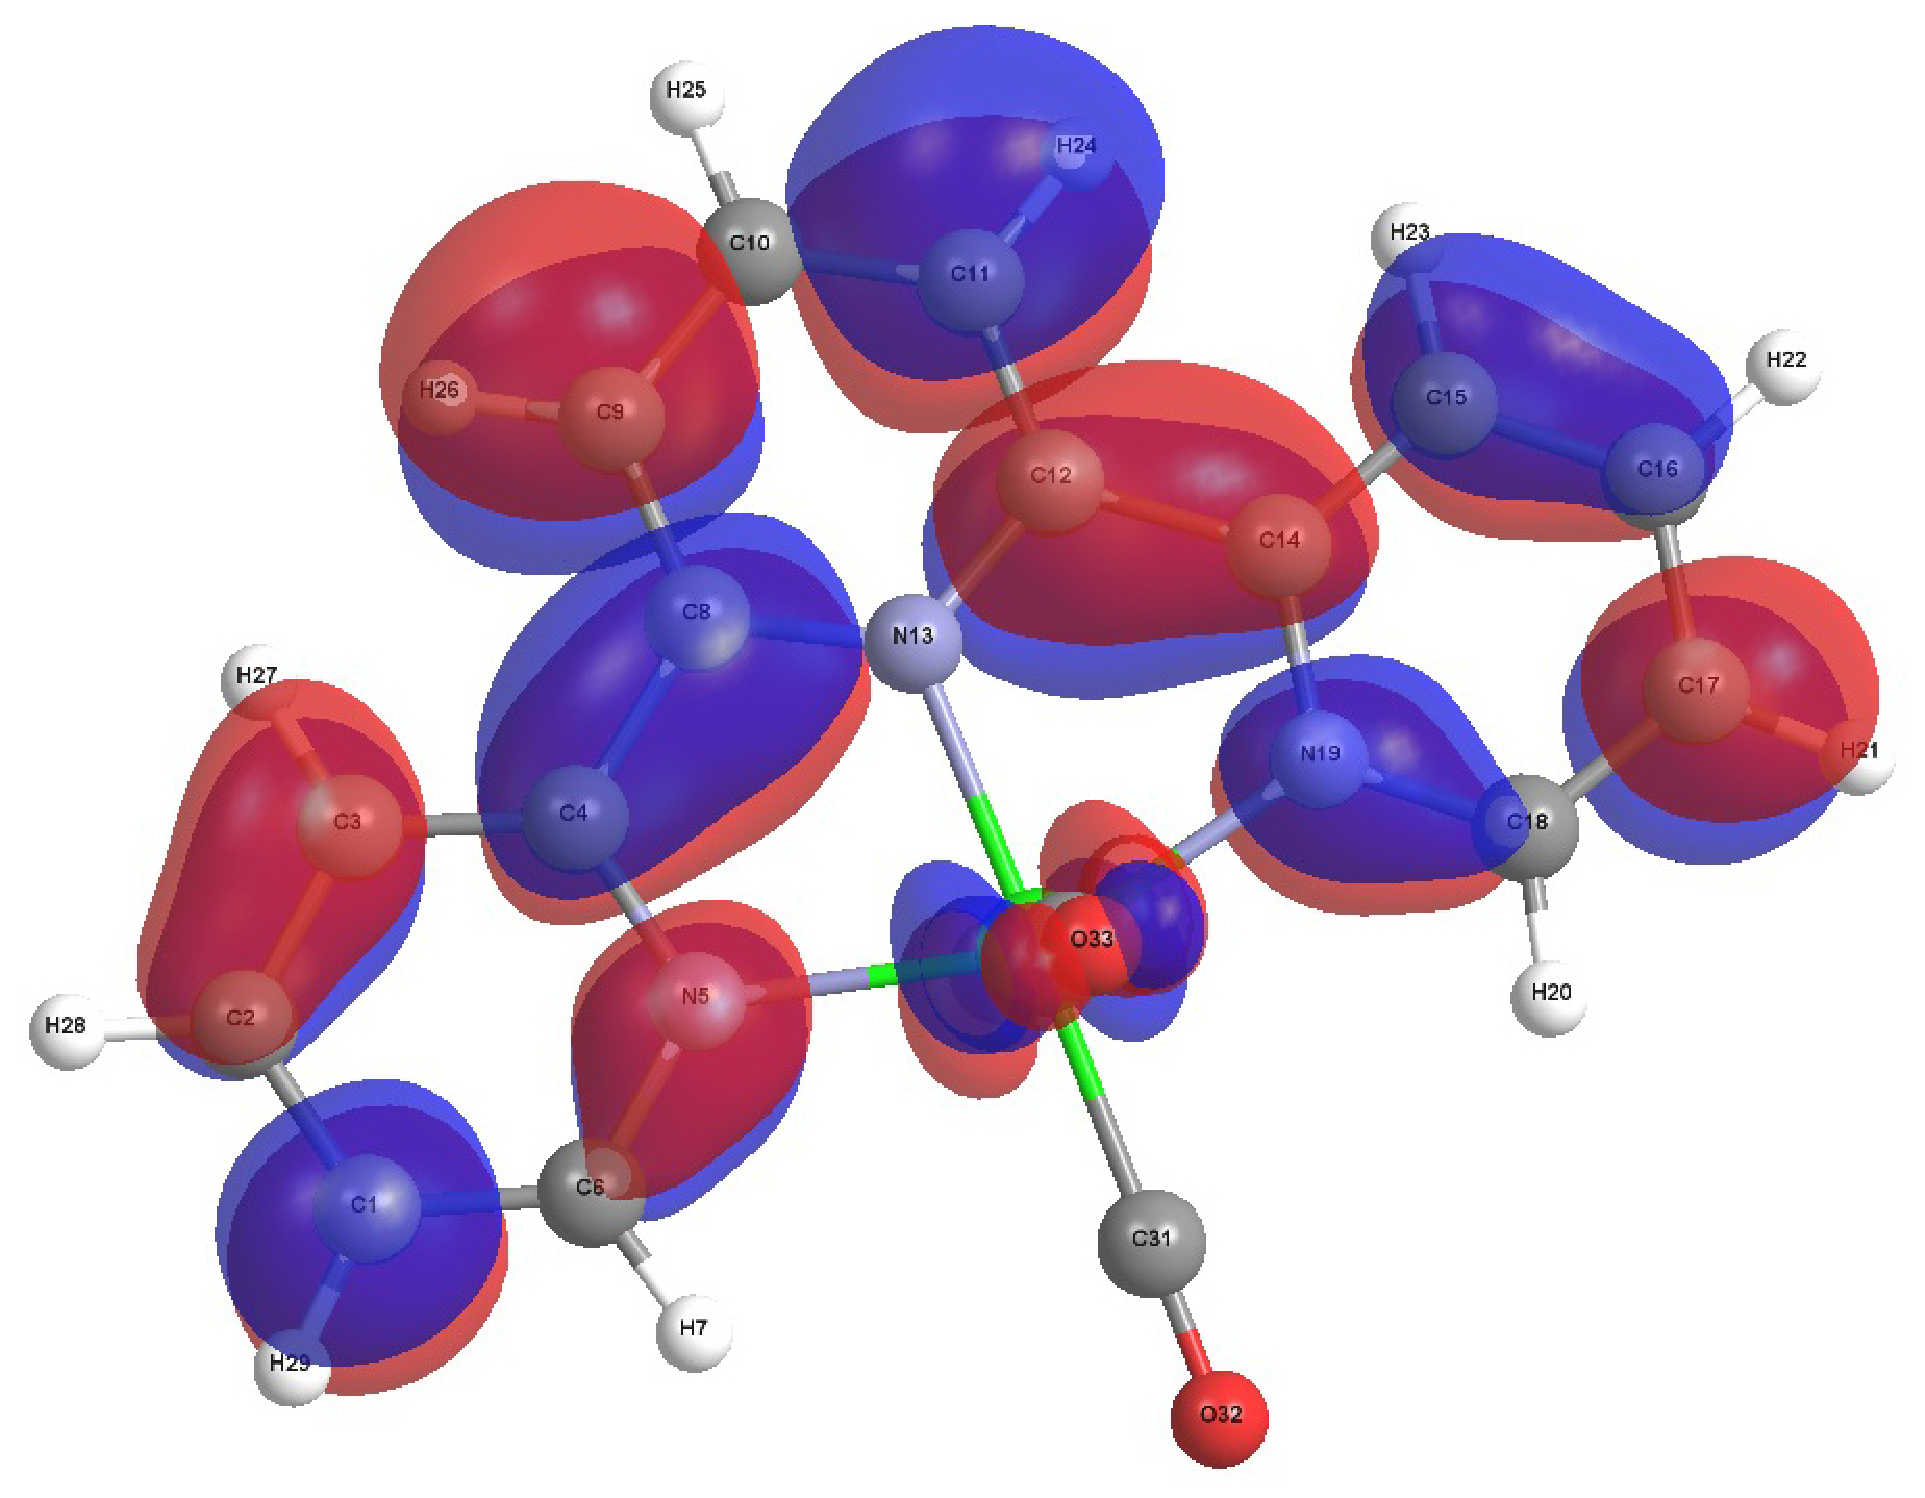
\includegraphics[clip=true, width=\textwidth, keepaspectratio]{images/mos/2l+1.eps}
  \caption{LUMO+1}
 \end{subfigure}
  \begin{subfigure}[b]{0.31\textwidth}
  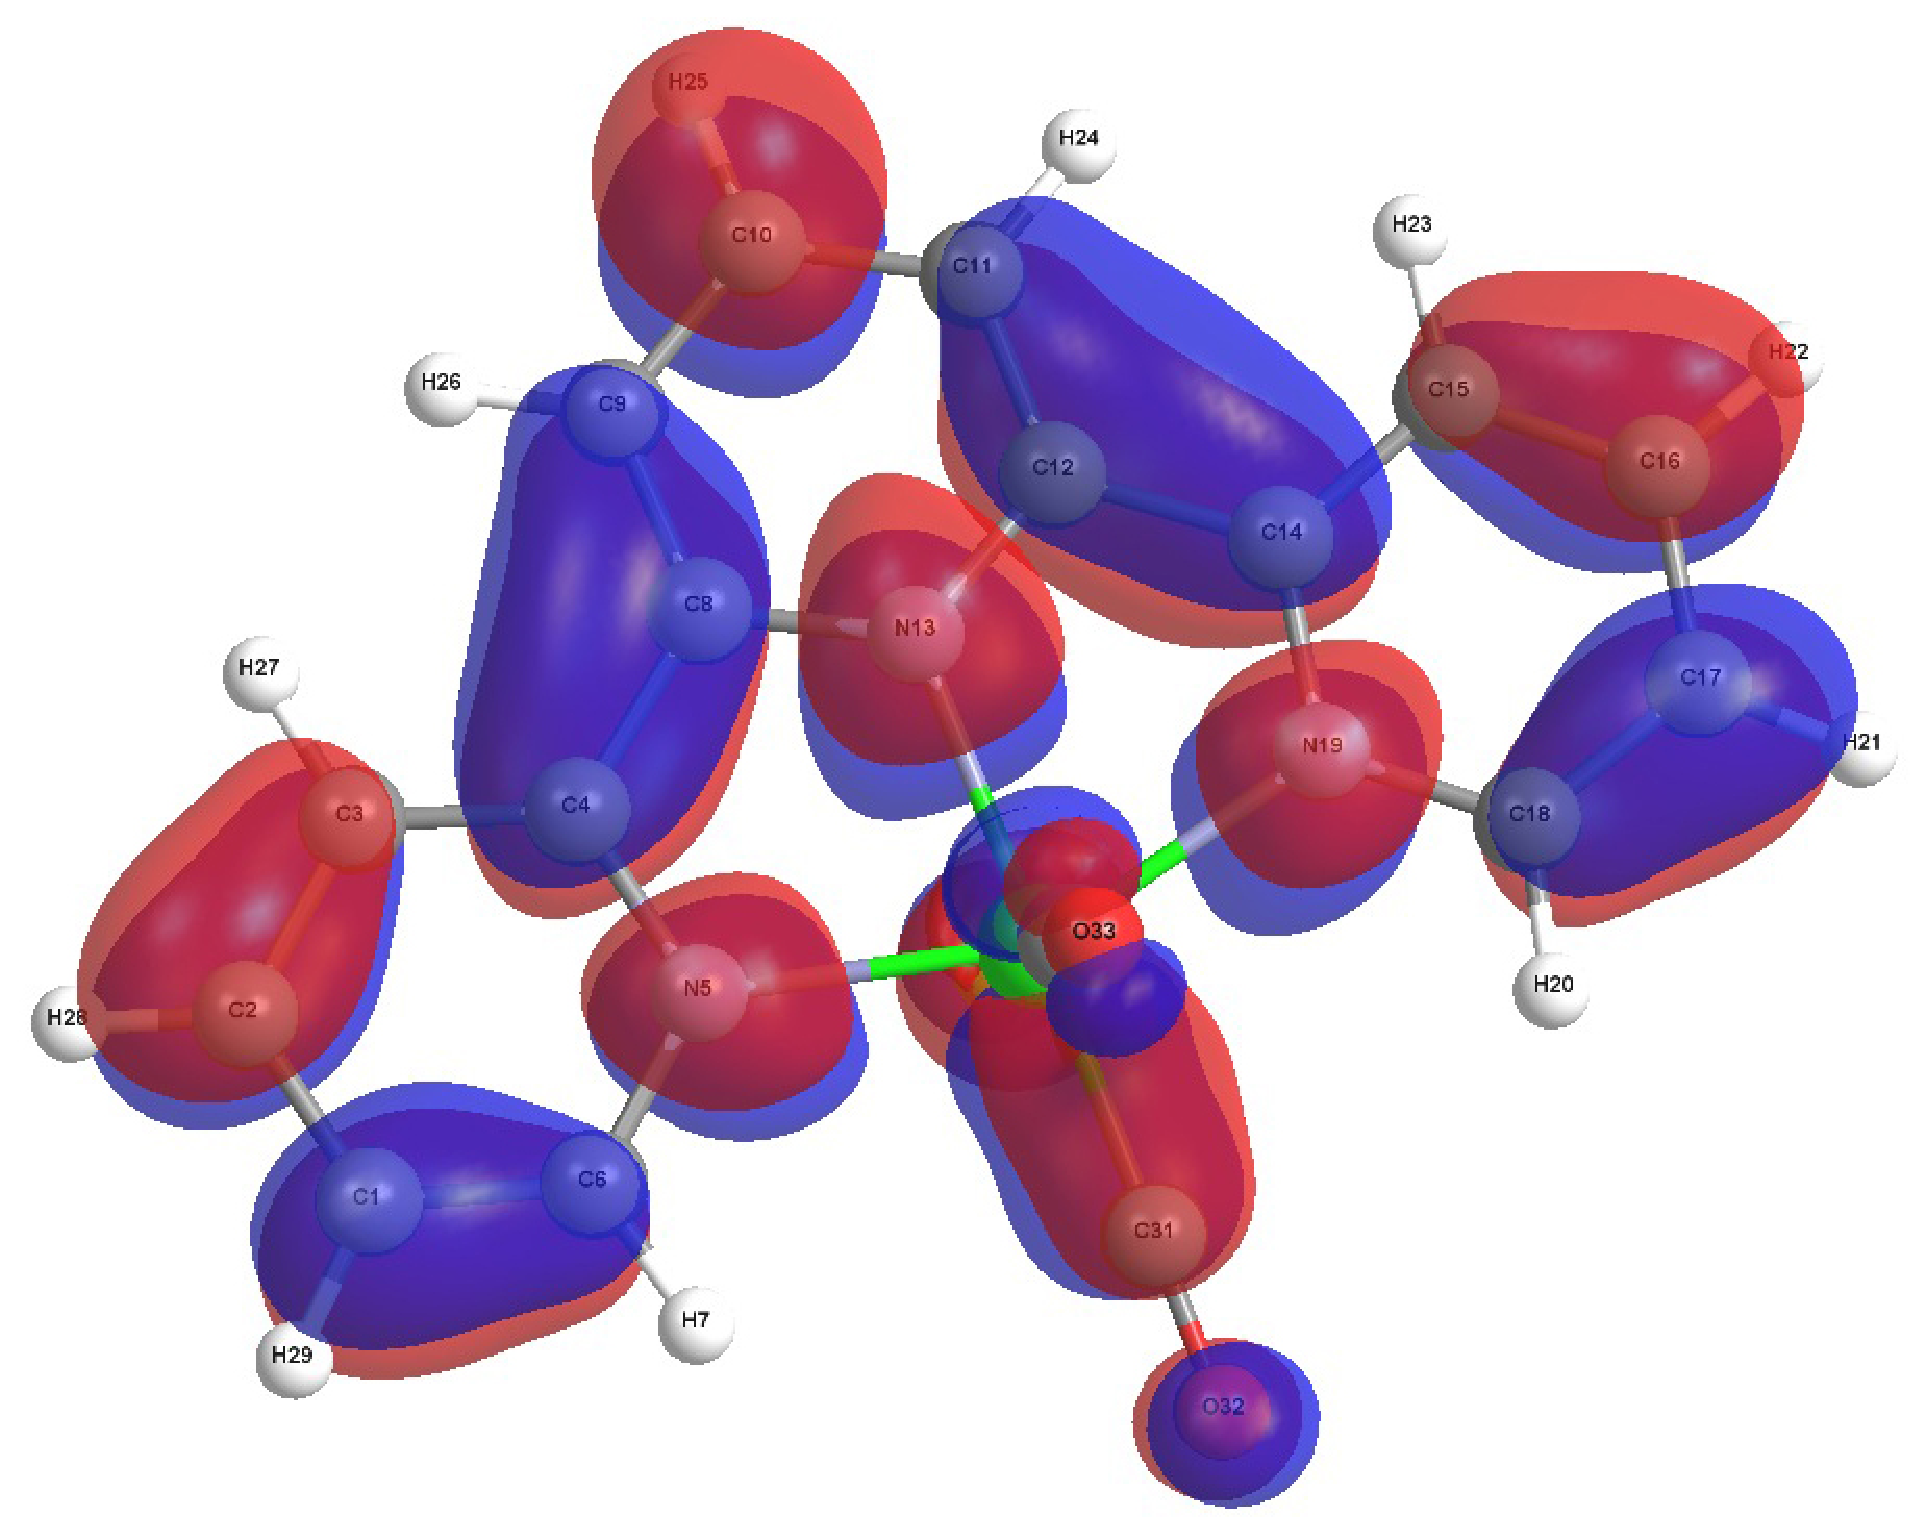
\includegraphics[clip=true, width=\textwidth, keepaspectratio]{images/mos/2l.eps}
  \caption{LUMO}
 \end{subfigure}
 \begin{subfigure}[b]{0.31\textwidth}
  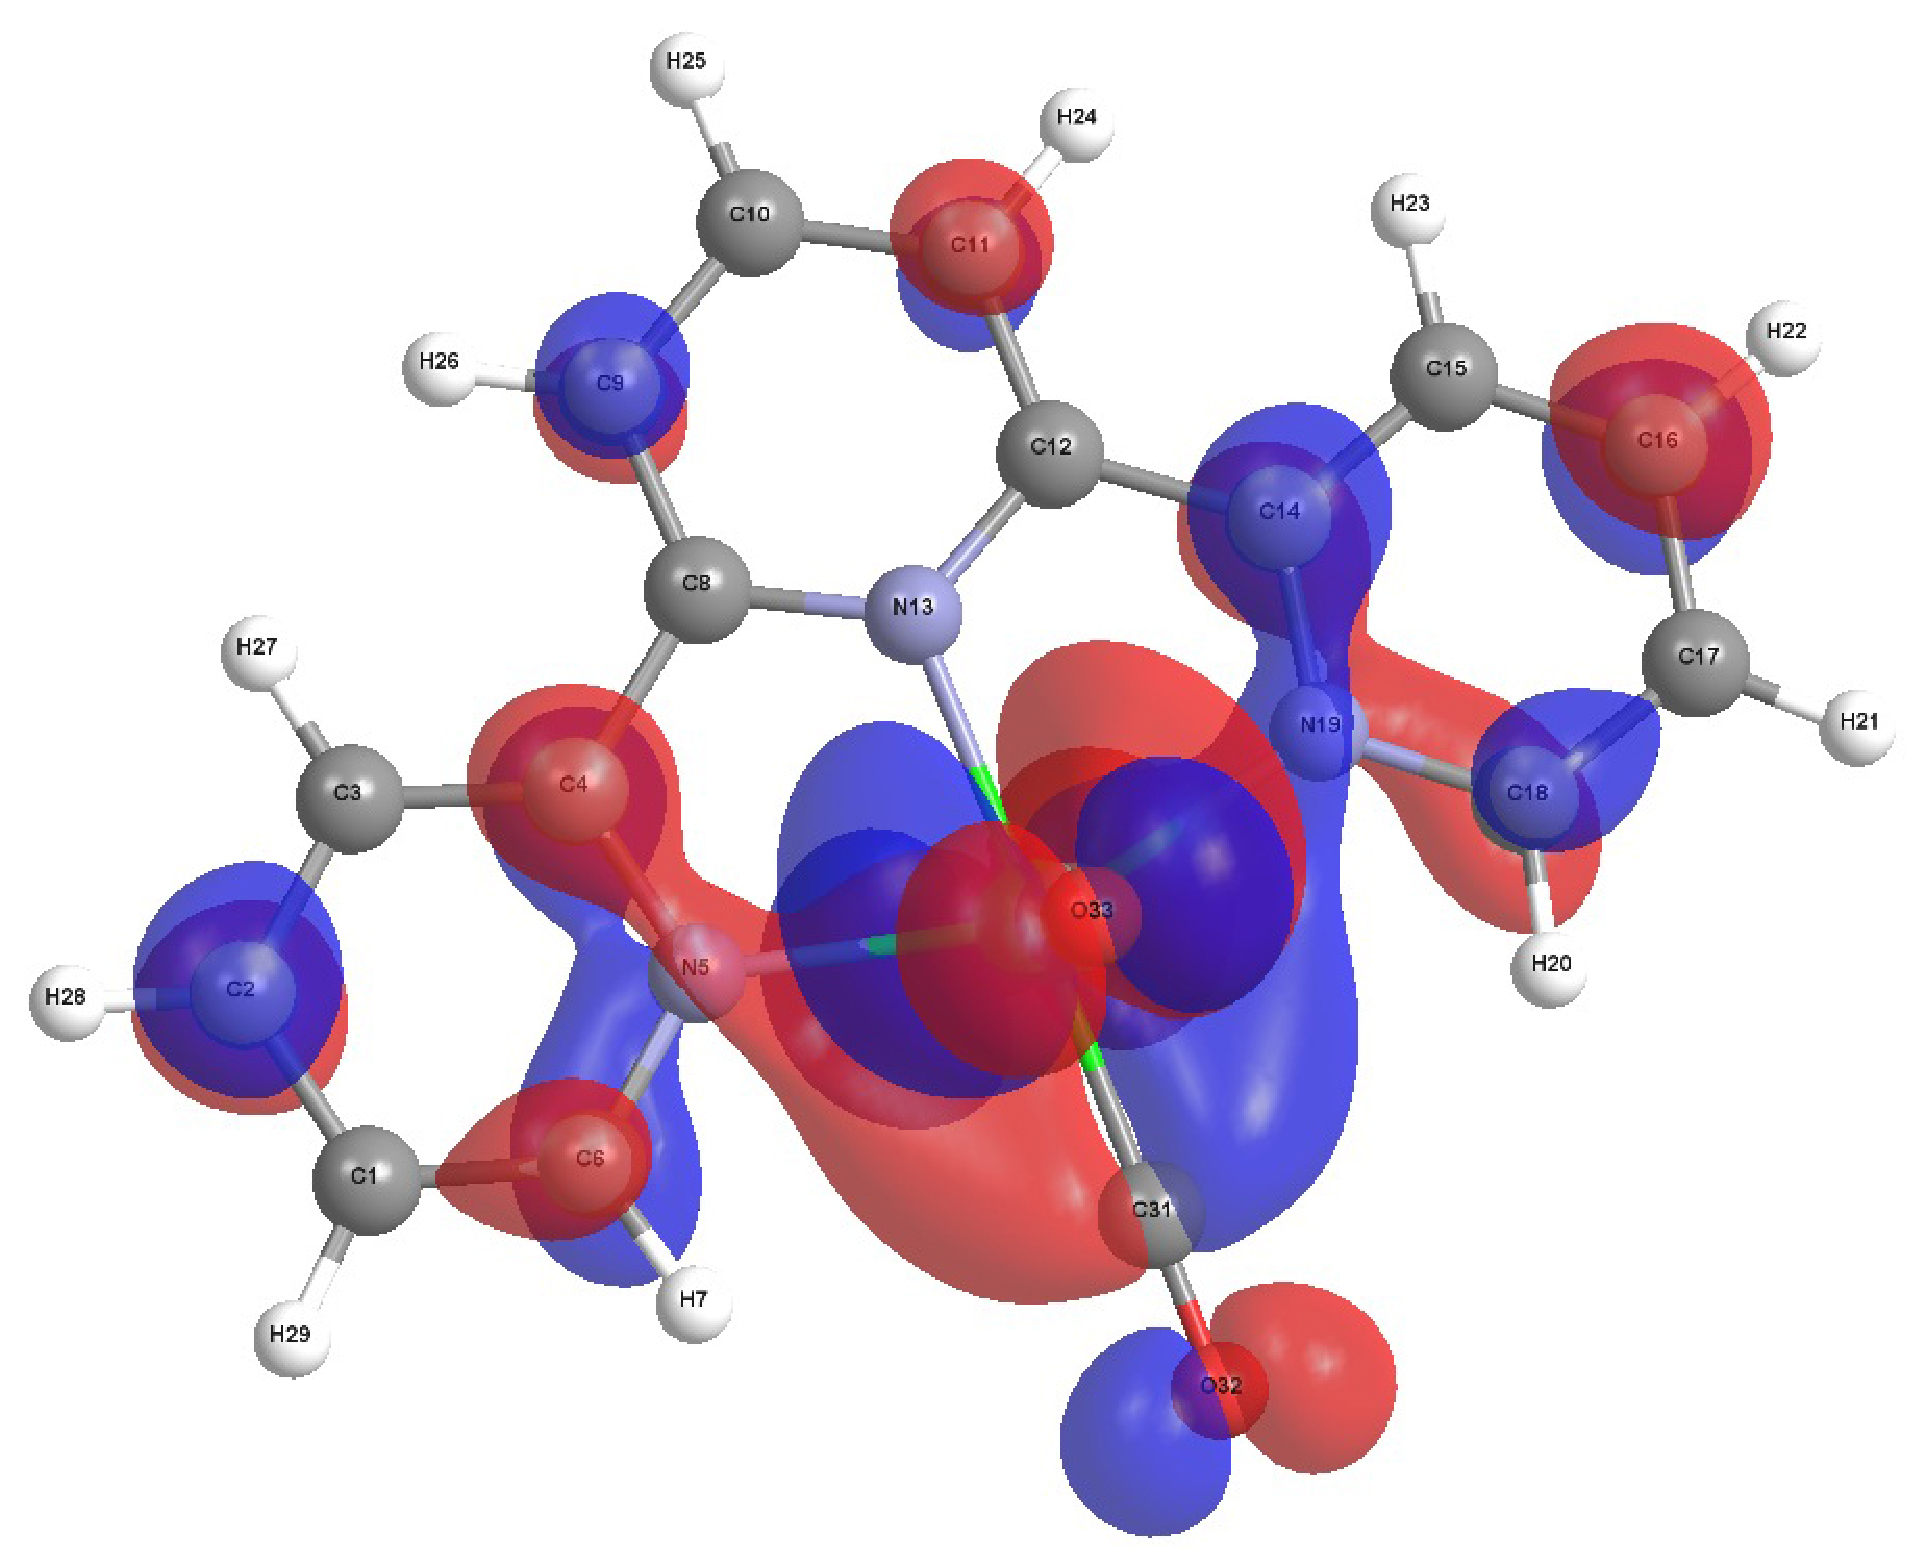
\includegraphics[clip=true, width=\textwidth, keepaspectratio]{images/mos/2h.eps}
  \caption{HOMO}
 \end{subfigure}
 \begin{subfigure}[b]{0.31\textwidth}
  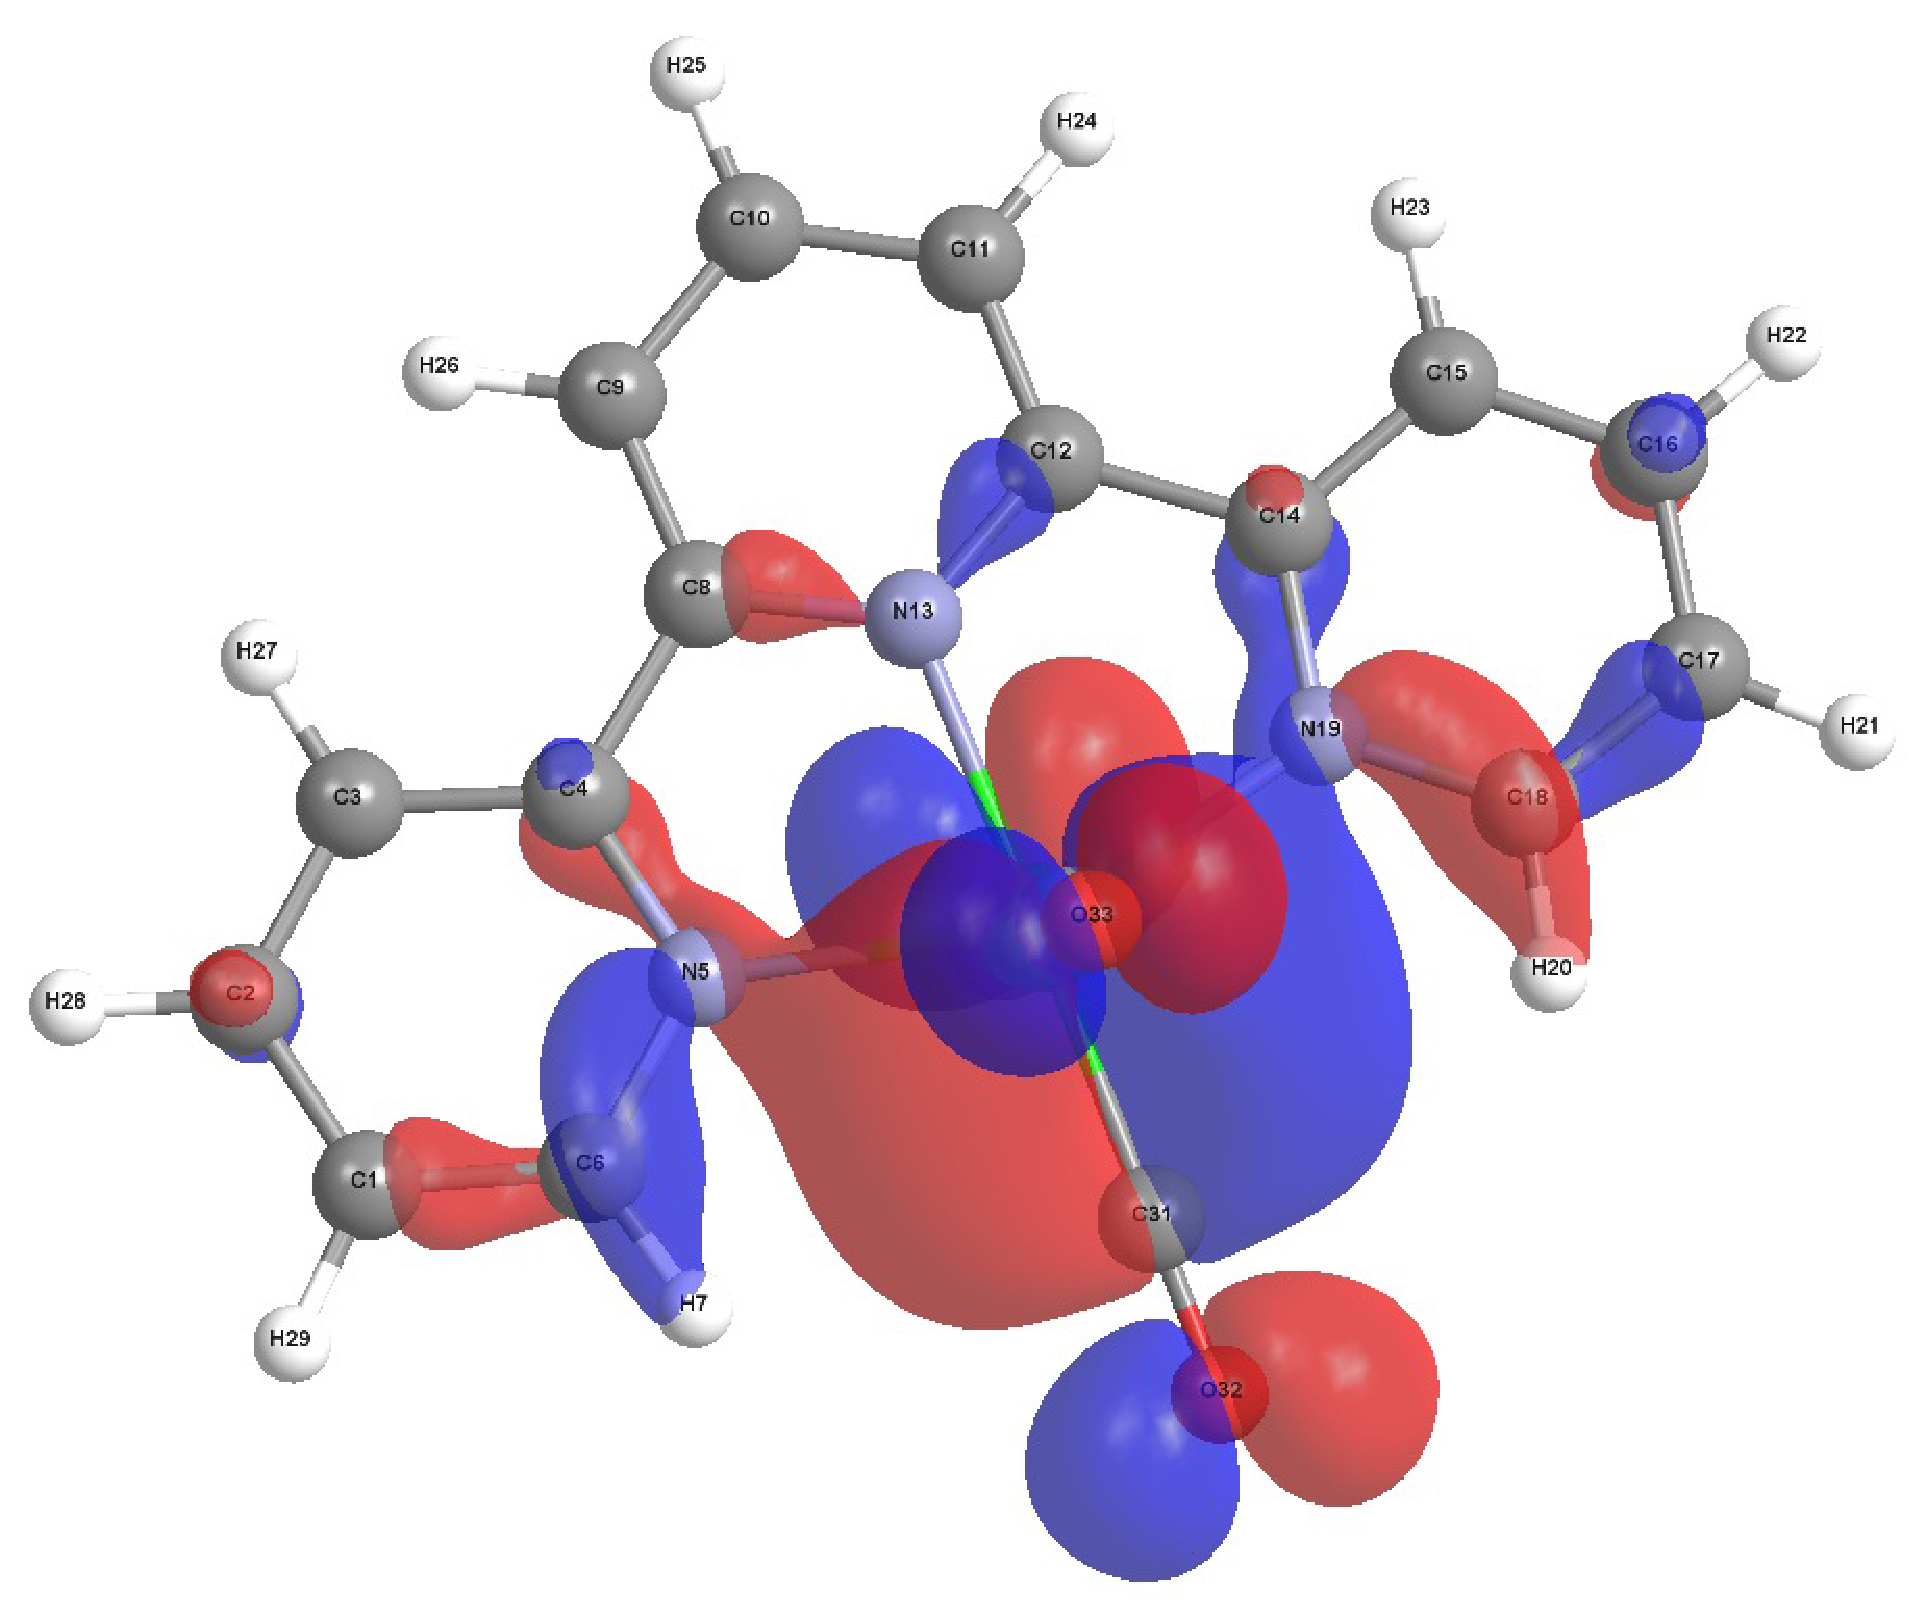
\includegraphics[clip=true, width=\textwidth, keepaspectratio]{images/mos/2h-1.eps}
  \caption{HOMO-1}
 \end{subfigure}
 \begin{subfigure}[b]{0.31\textwidth}
  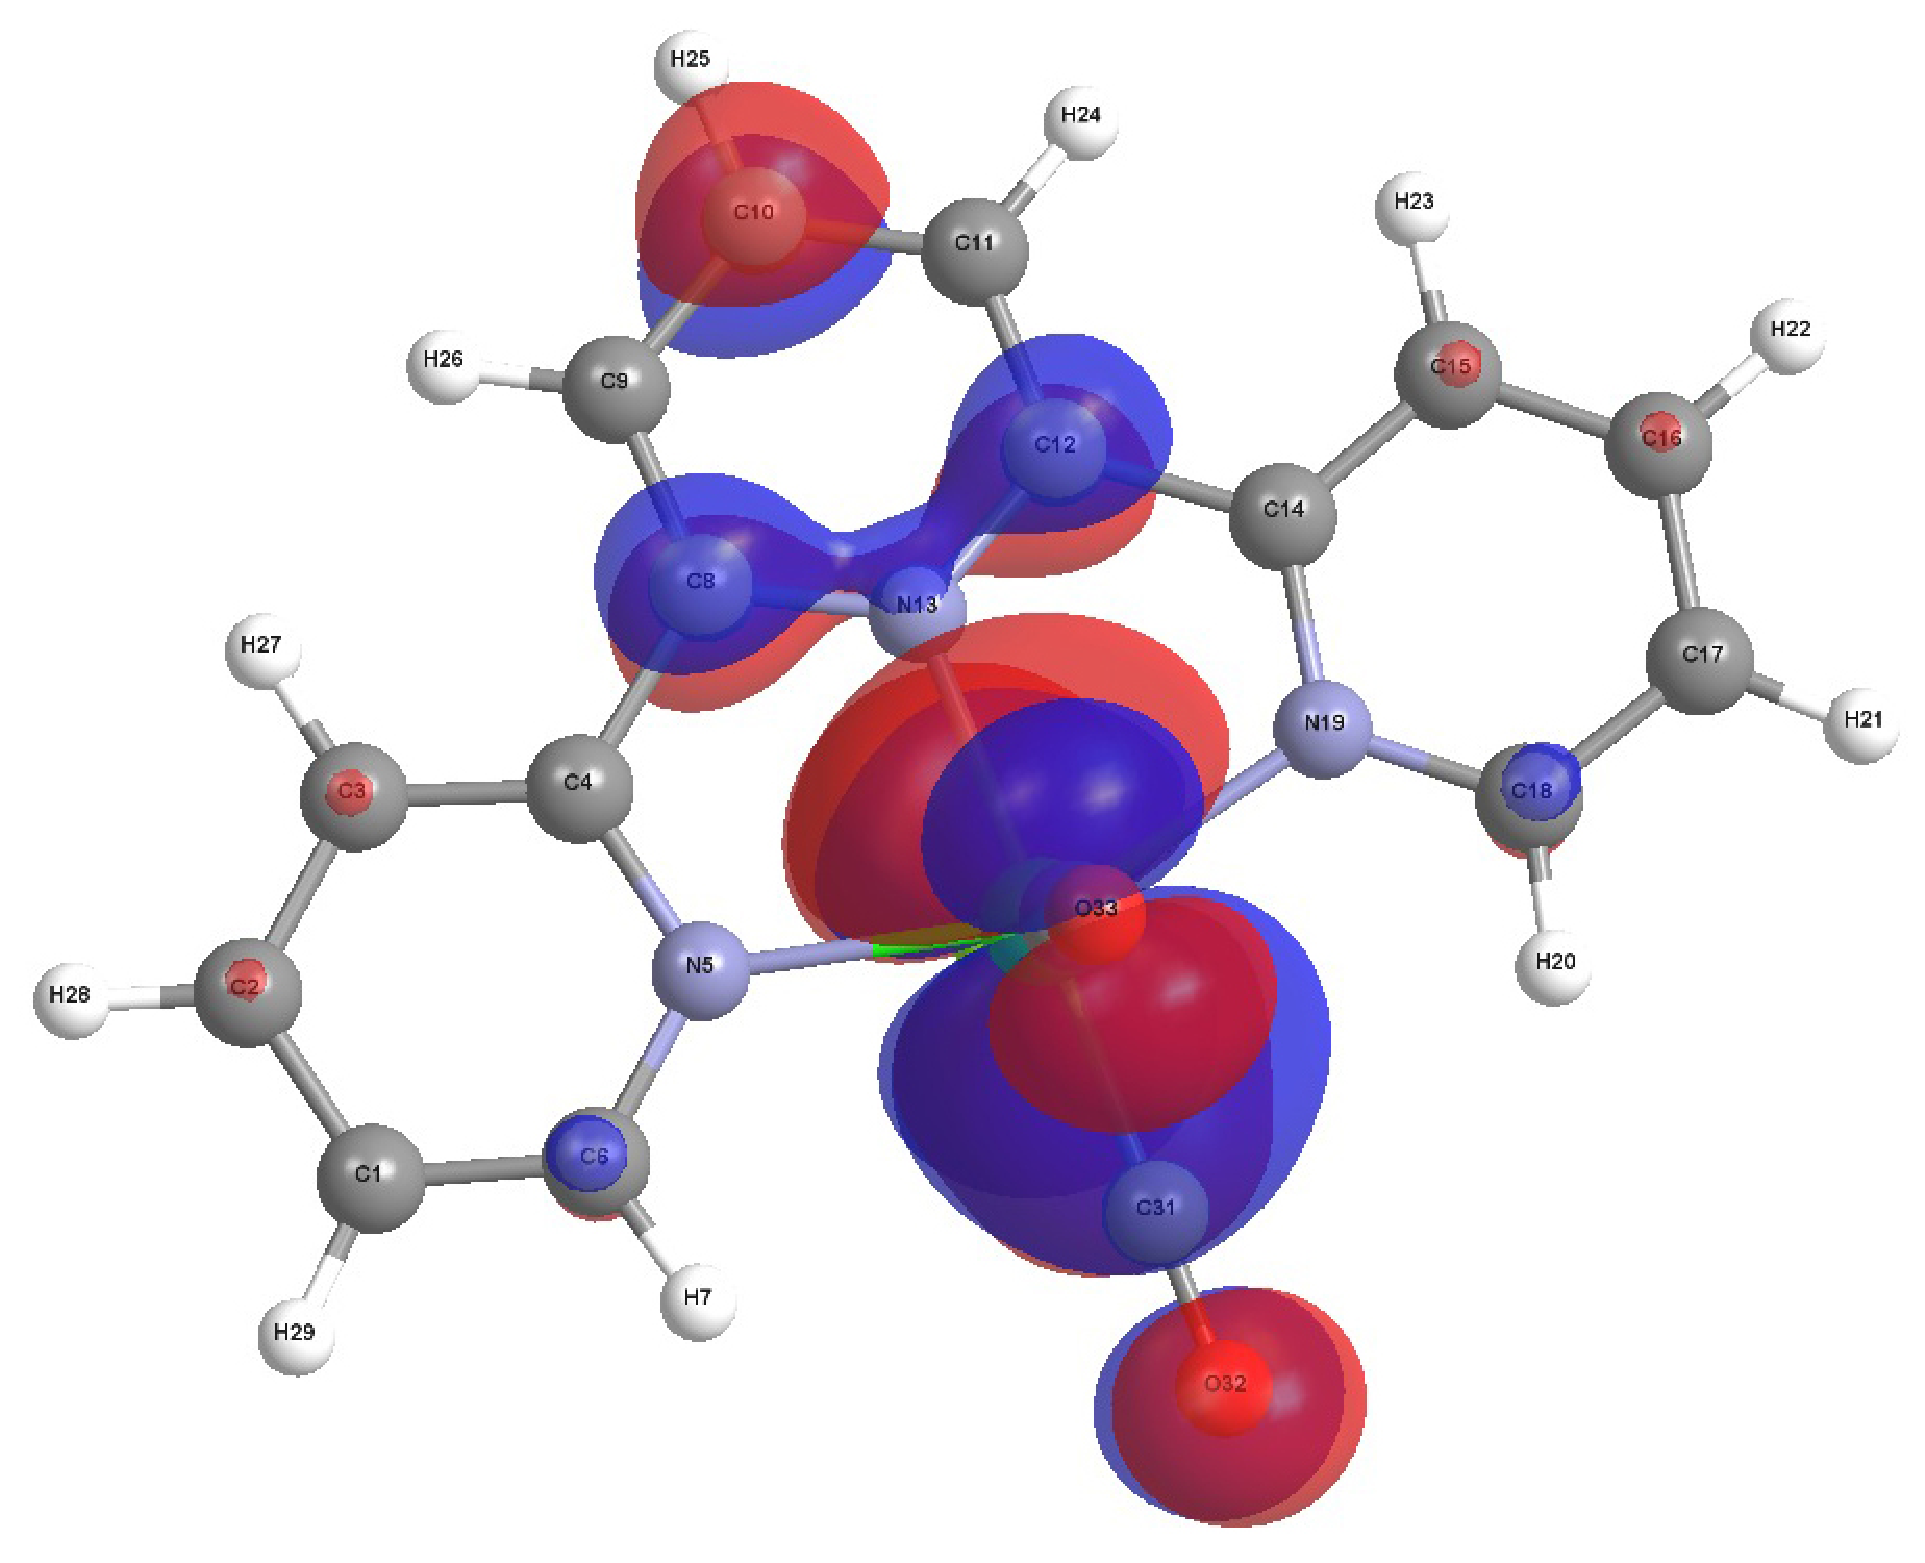
\includegraphics[clip=true, width=\textwidth, keepaspectratio]{images/mos/2h-2.eps}
  \caption{HOMO-2}
 \end{subfigure}
 \begin{subfigure}[b]{0.31\textwidth}
  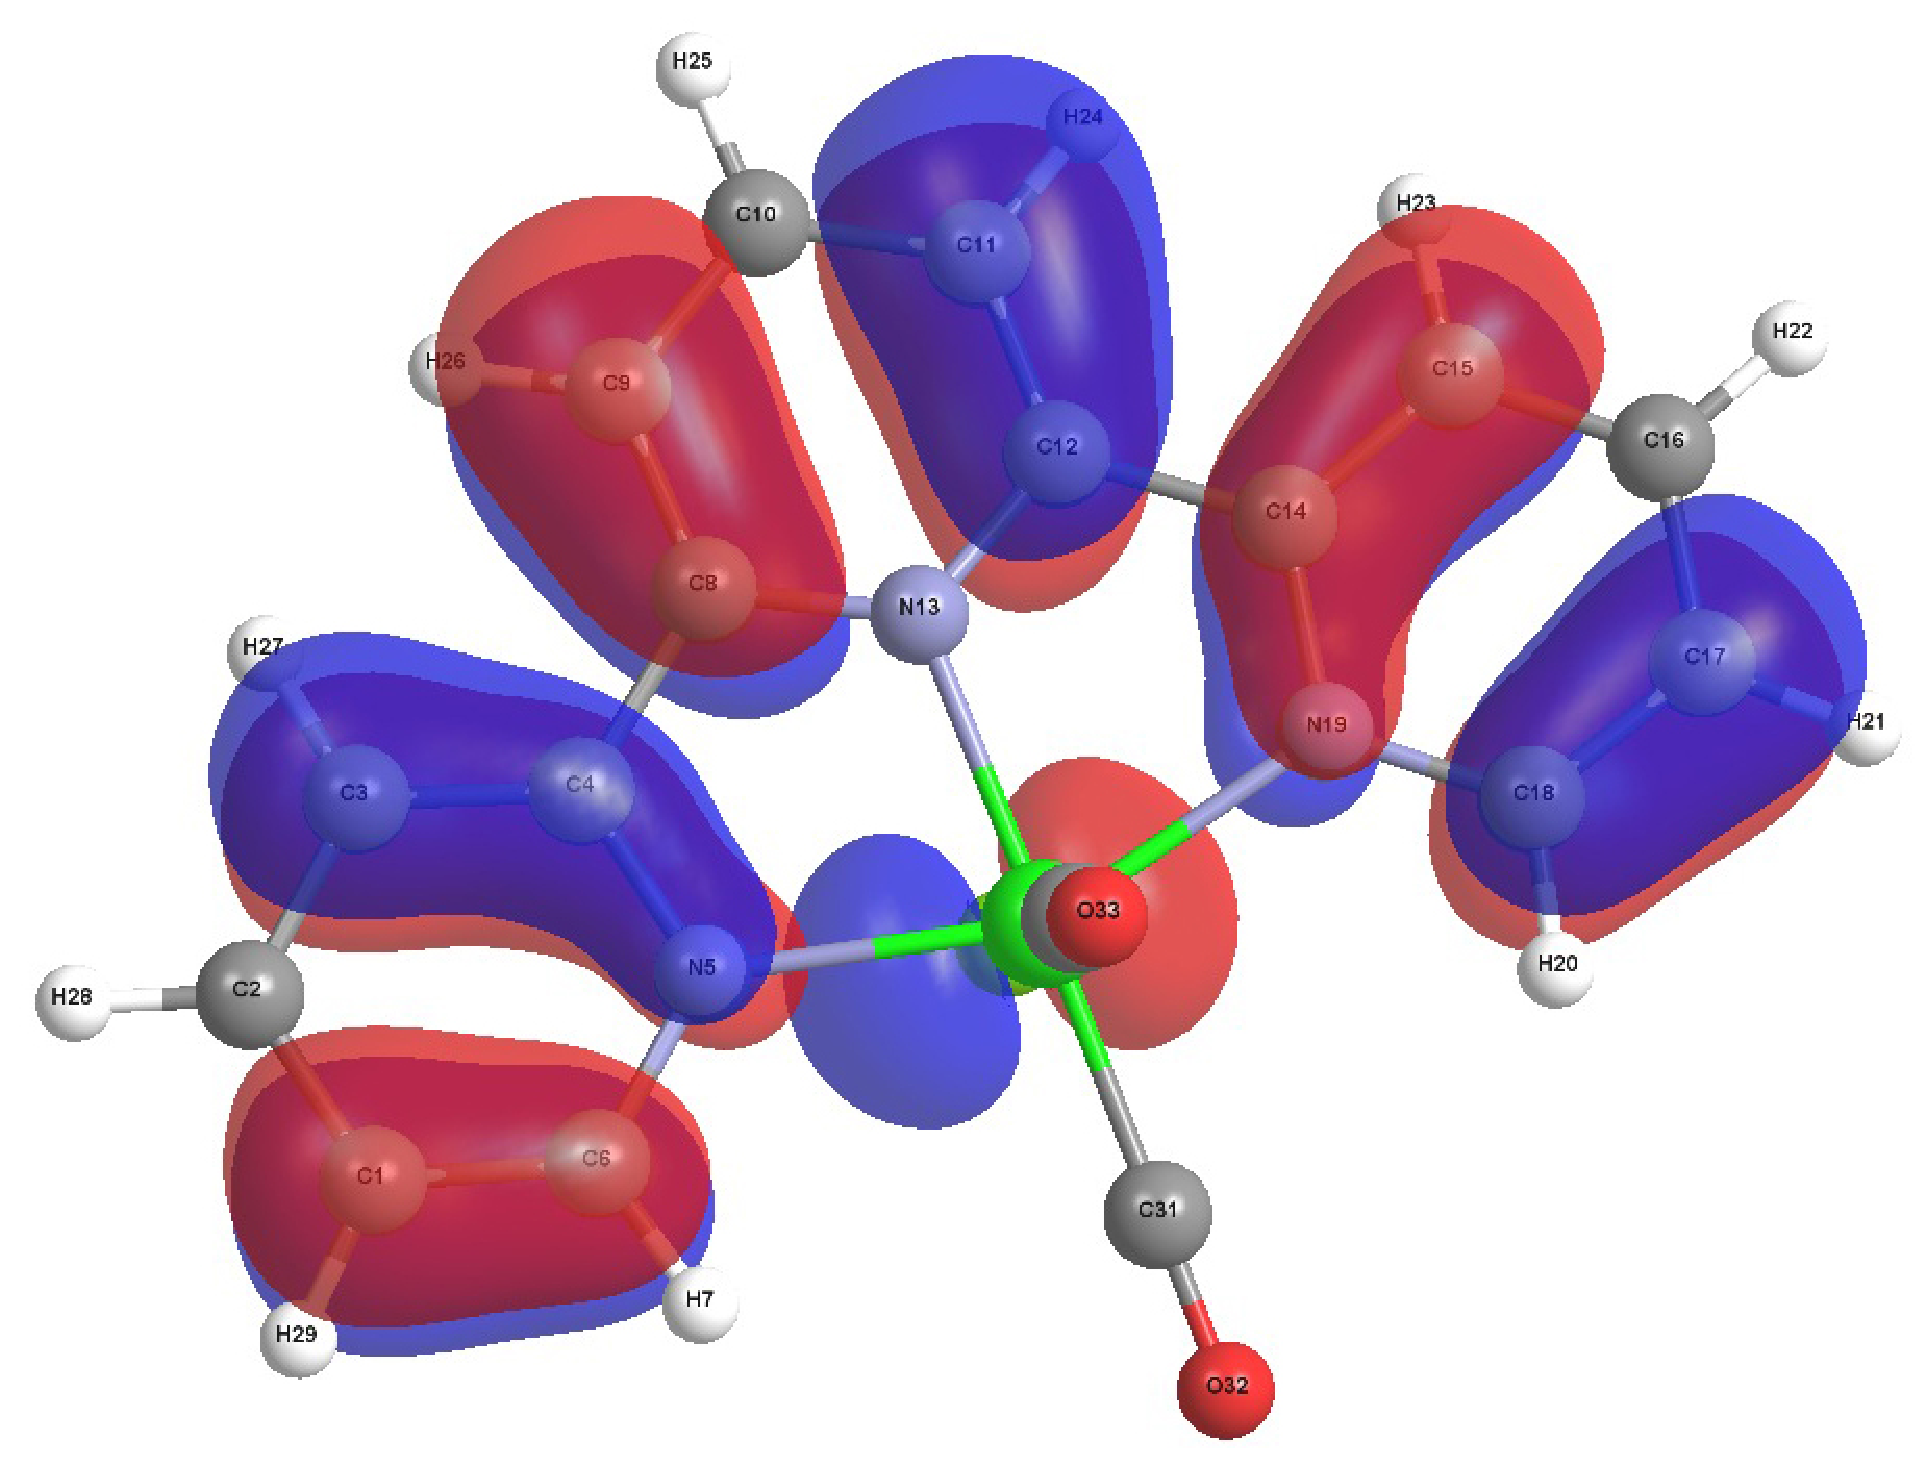
\includegraphics[clip=true, width=\textwidth, keepaspectratio]{images/mos/2h-3.eps}
  \caption{HOMO-3}
 \end{subfigure}
 \begin{subfigure}[b]{0.31\textwidth}
  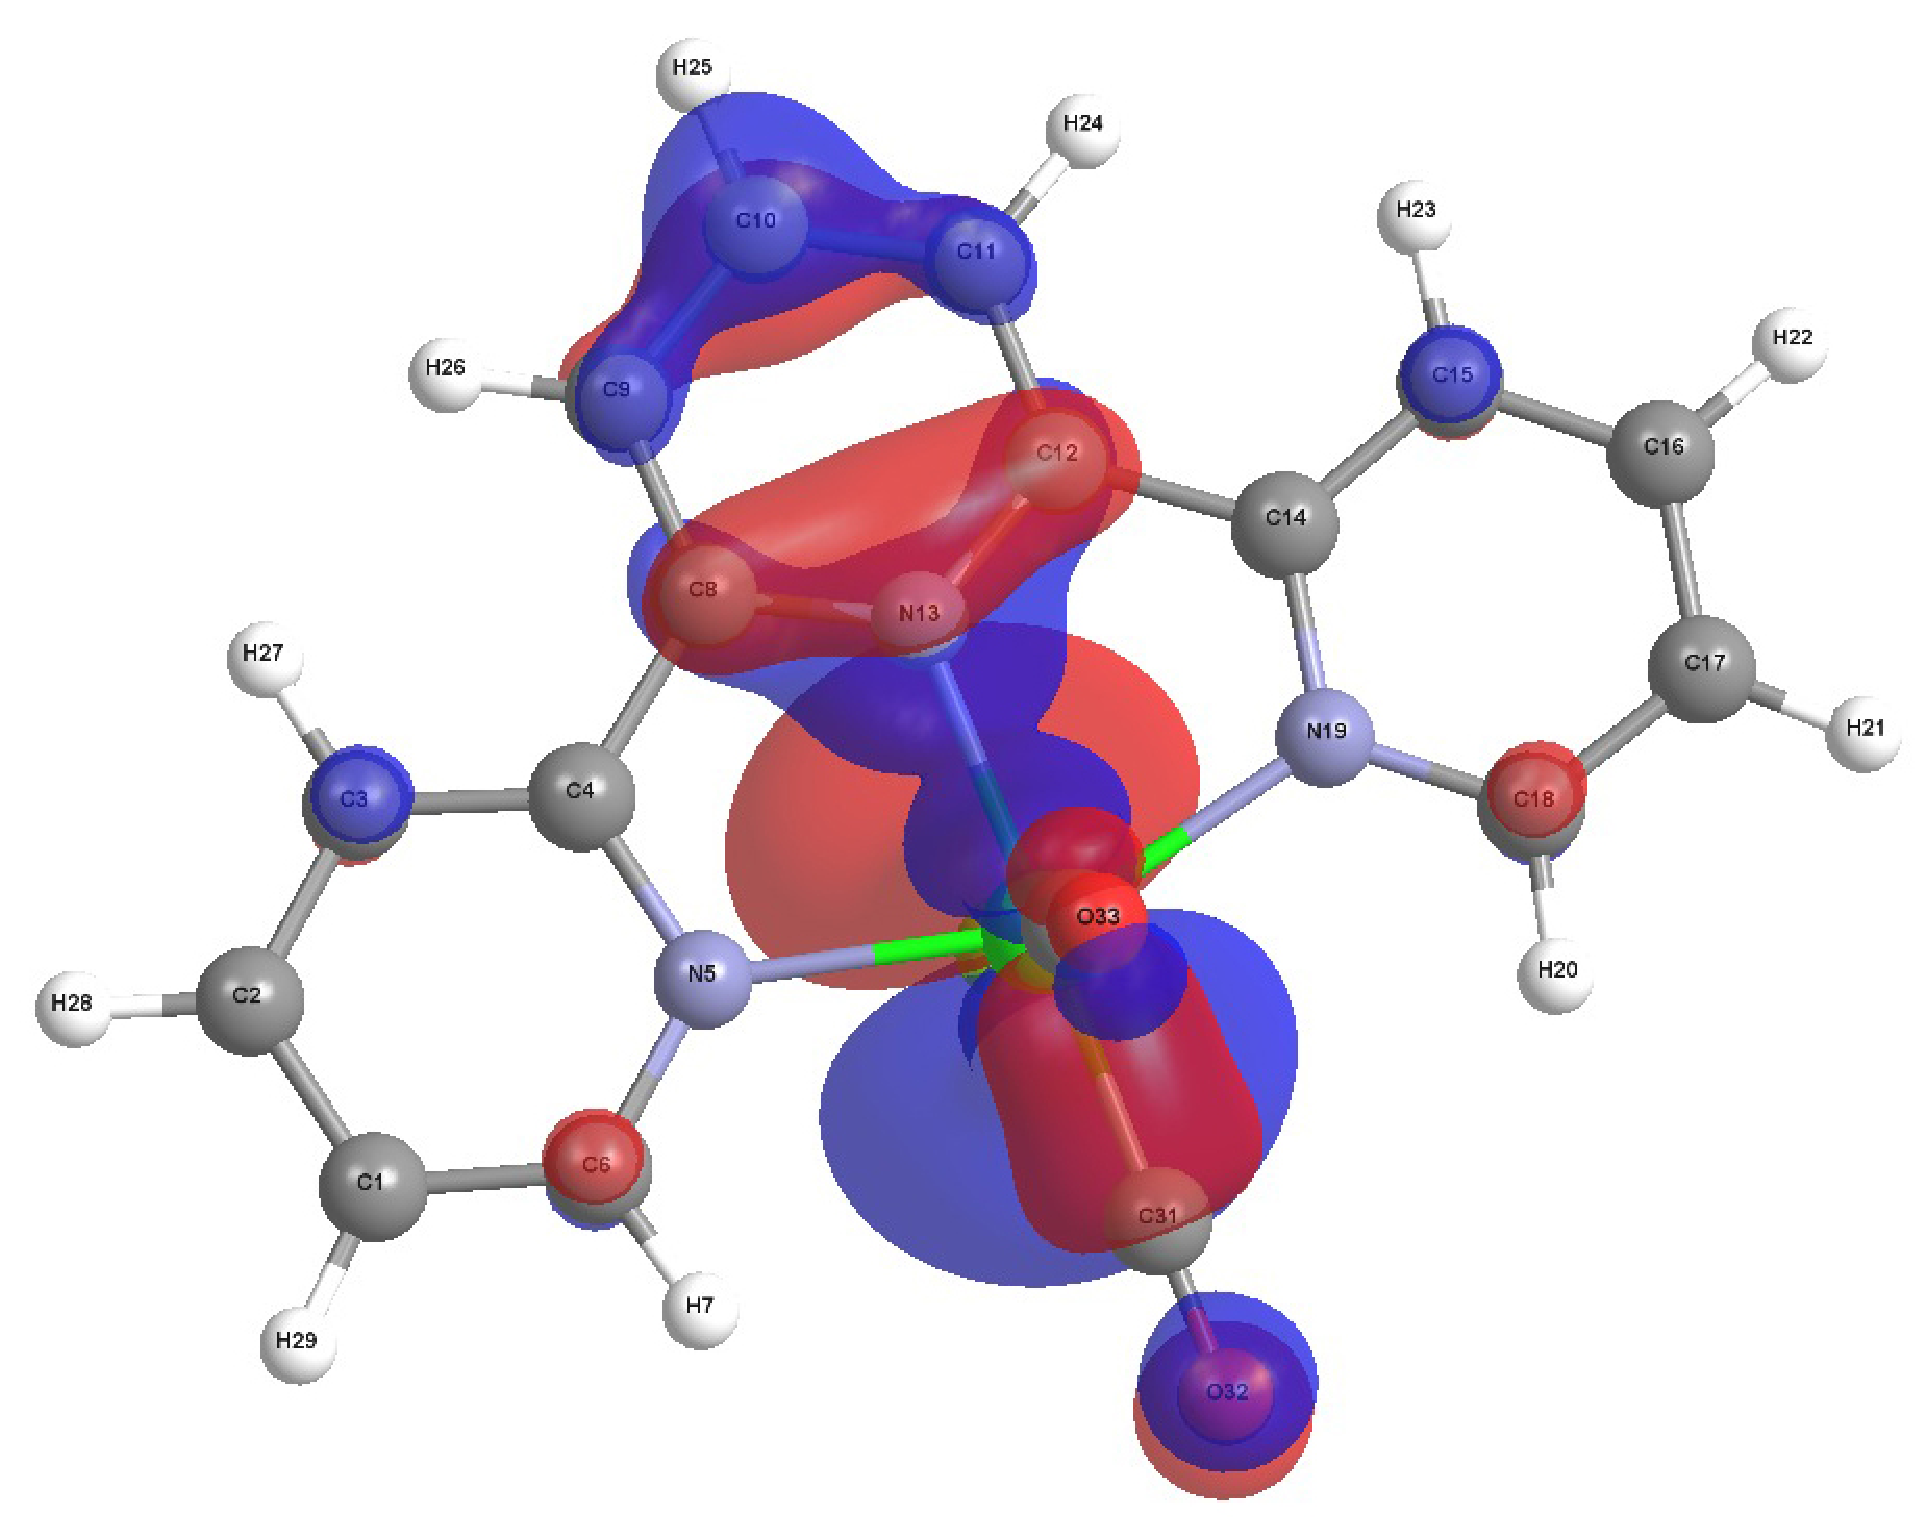
\includegraphics[clip=true, width=\textwidth, keepaspectratio]{images/mos/2h-4.eps}
  \caption{HOMO-5}
 \end{subfigure}
 \begin{subfigure}[b]{0.31\textwidth}
  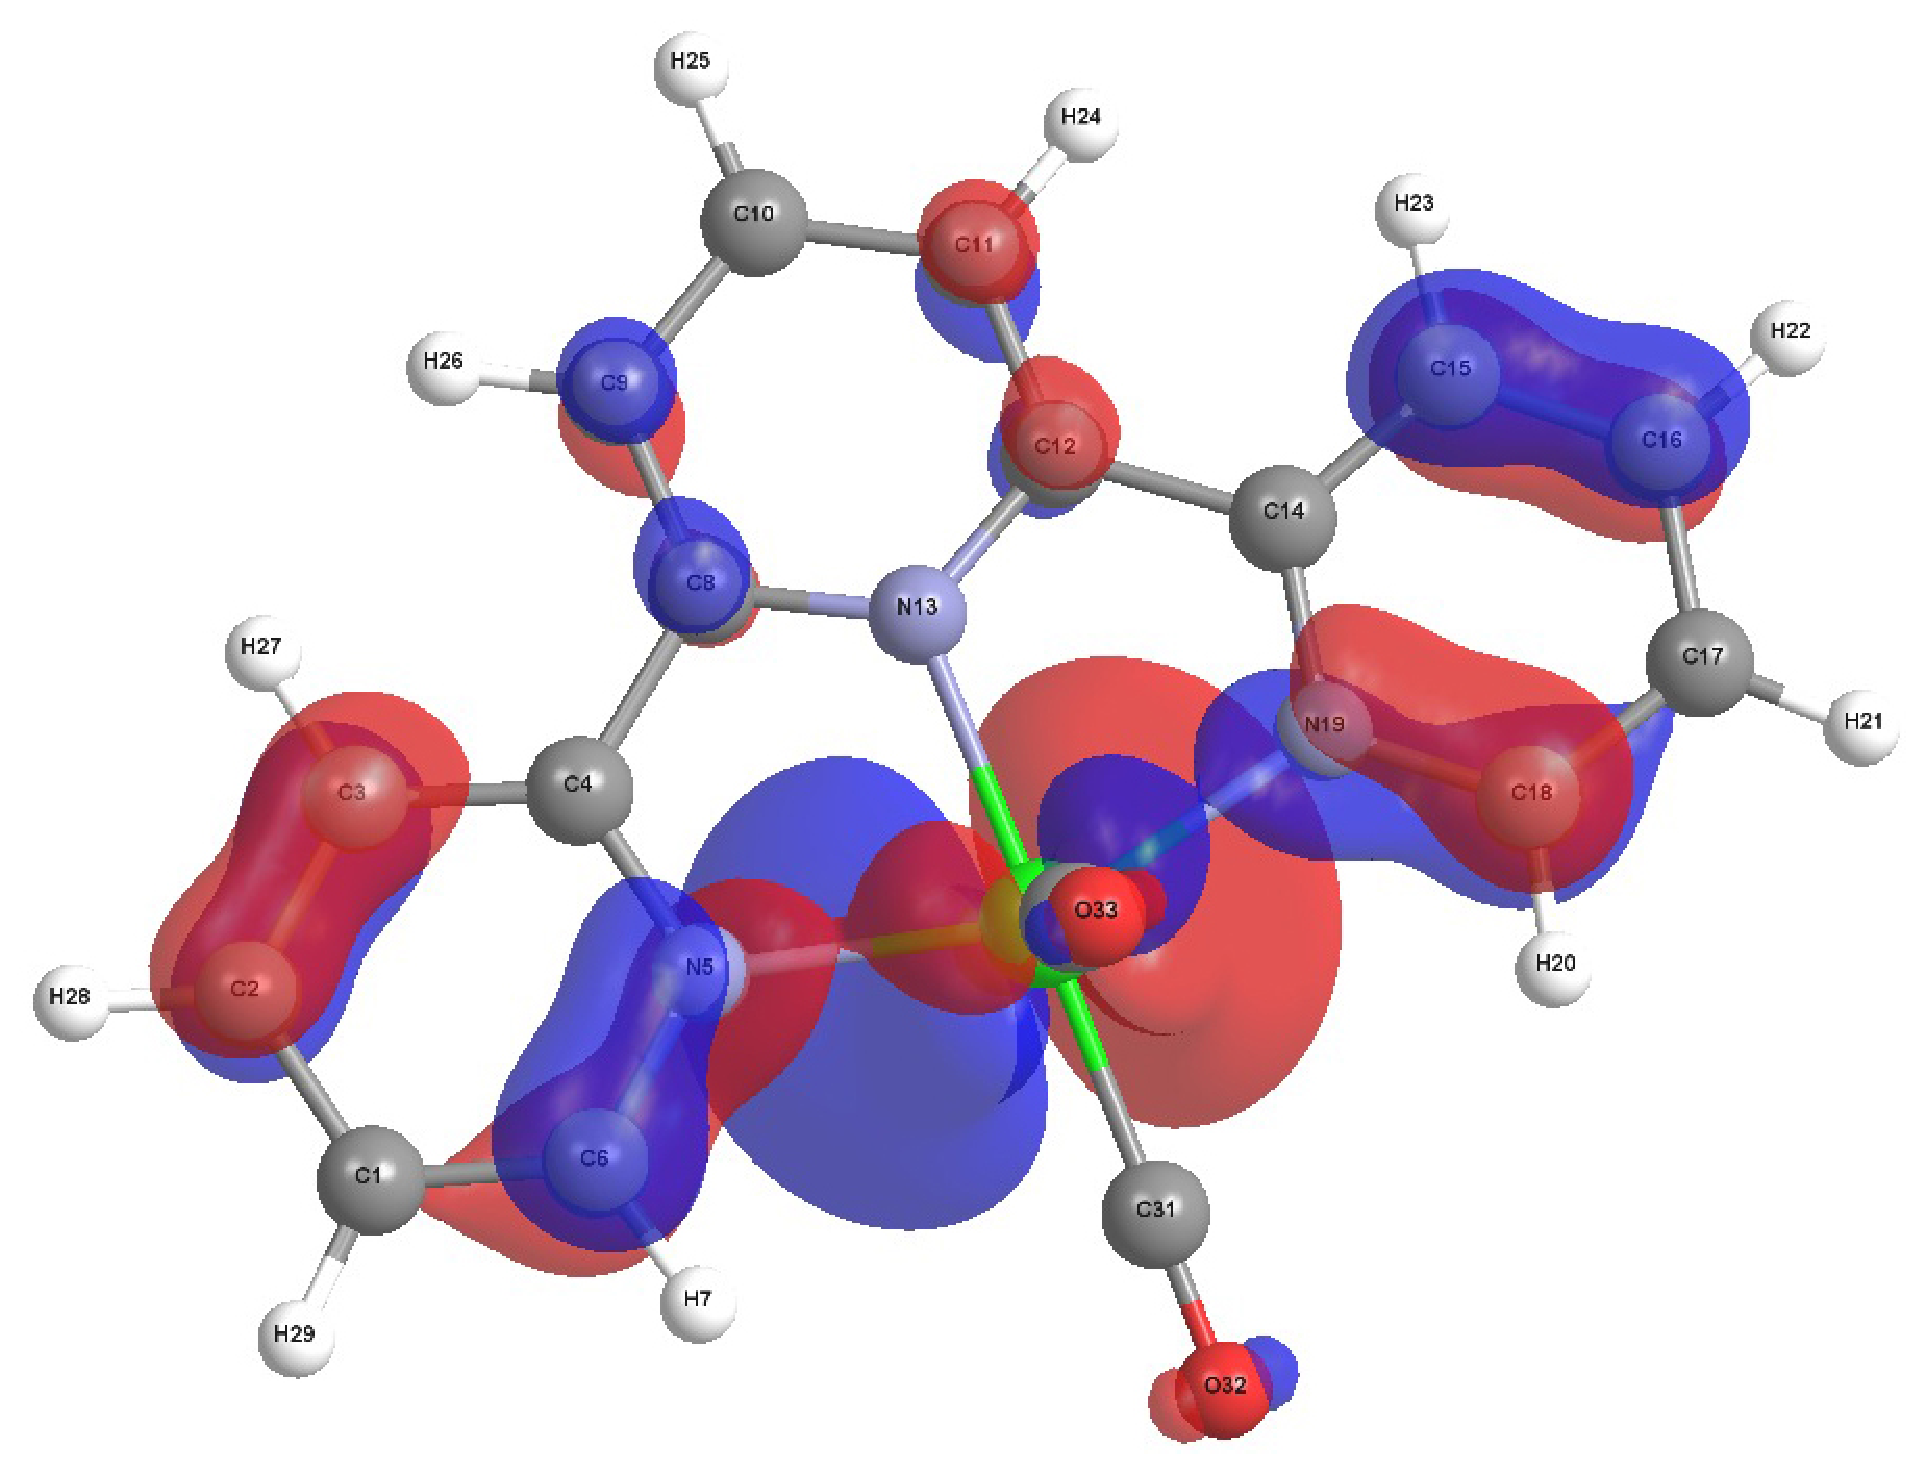
\includegraphics[clip=true, width=\textwidth, keepaspectratio]{images/mos/2h-5.eps}
  \caption{HOMO-5}
 \end{subfigure}
\caption[Molecular orbitals HOMO-5 to LUMO+3 of \textbf{2.2}]{Isosurface plots of the frontier molecular orbitals HOMO-5 to LUMO+3 of \textbf{2.2}}
\label{fig.mo22}
\end{figure} 

\begin{figure}[!ht]
 \centering
 \begin{subfigure}[b]{0.31\textwidth}
  \includegraphics[clip=true, width=\textwidth, keepaspectratio]{images/mos/3l+2.eps}
  \caption{LUMO+2}
 \end{subfigure}
  \begin{subfigure}[b]{0.31\textwidth}
  \includegraphics[clip=true, width=\textwidth, keepaspectratio]{images/mos/3l+1.eps}
  \caption{LUMO+1}
 \end{subfigure}
  \begin{subfigure}[b]{0.31\textwidth}
  \includegraphics[clip=true, width=\textwidth, keepaspectratio]{images/mos/3l.eps}
  \caption{LUMO}
 \end{subfigure}
 \begin{subfigure}[b]{0.31\textwidth}
  \includegraphics[clip=true, width=\textwidth, keepaspectratio]{images/mos/3h.eps}
  \caption{HOMO}
 \end{subfigure}
 \begin{subfigure}[b]{0.31\textwidth}
  \includegraphics[clip=true, width=\textwidth, keepaspectratio]{images/mos/3h-1.eps}
  \caption{HOMO-1}
 \end{subfigure}
 \begin{subfigure}[b]{0.31\textwidth}
  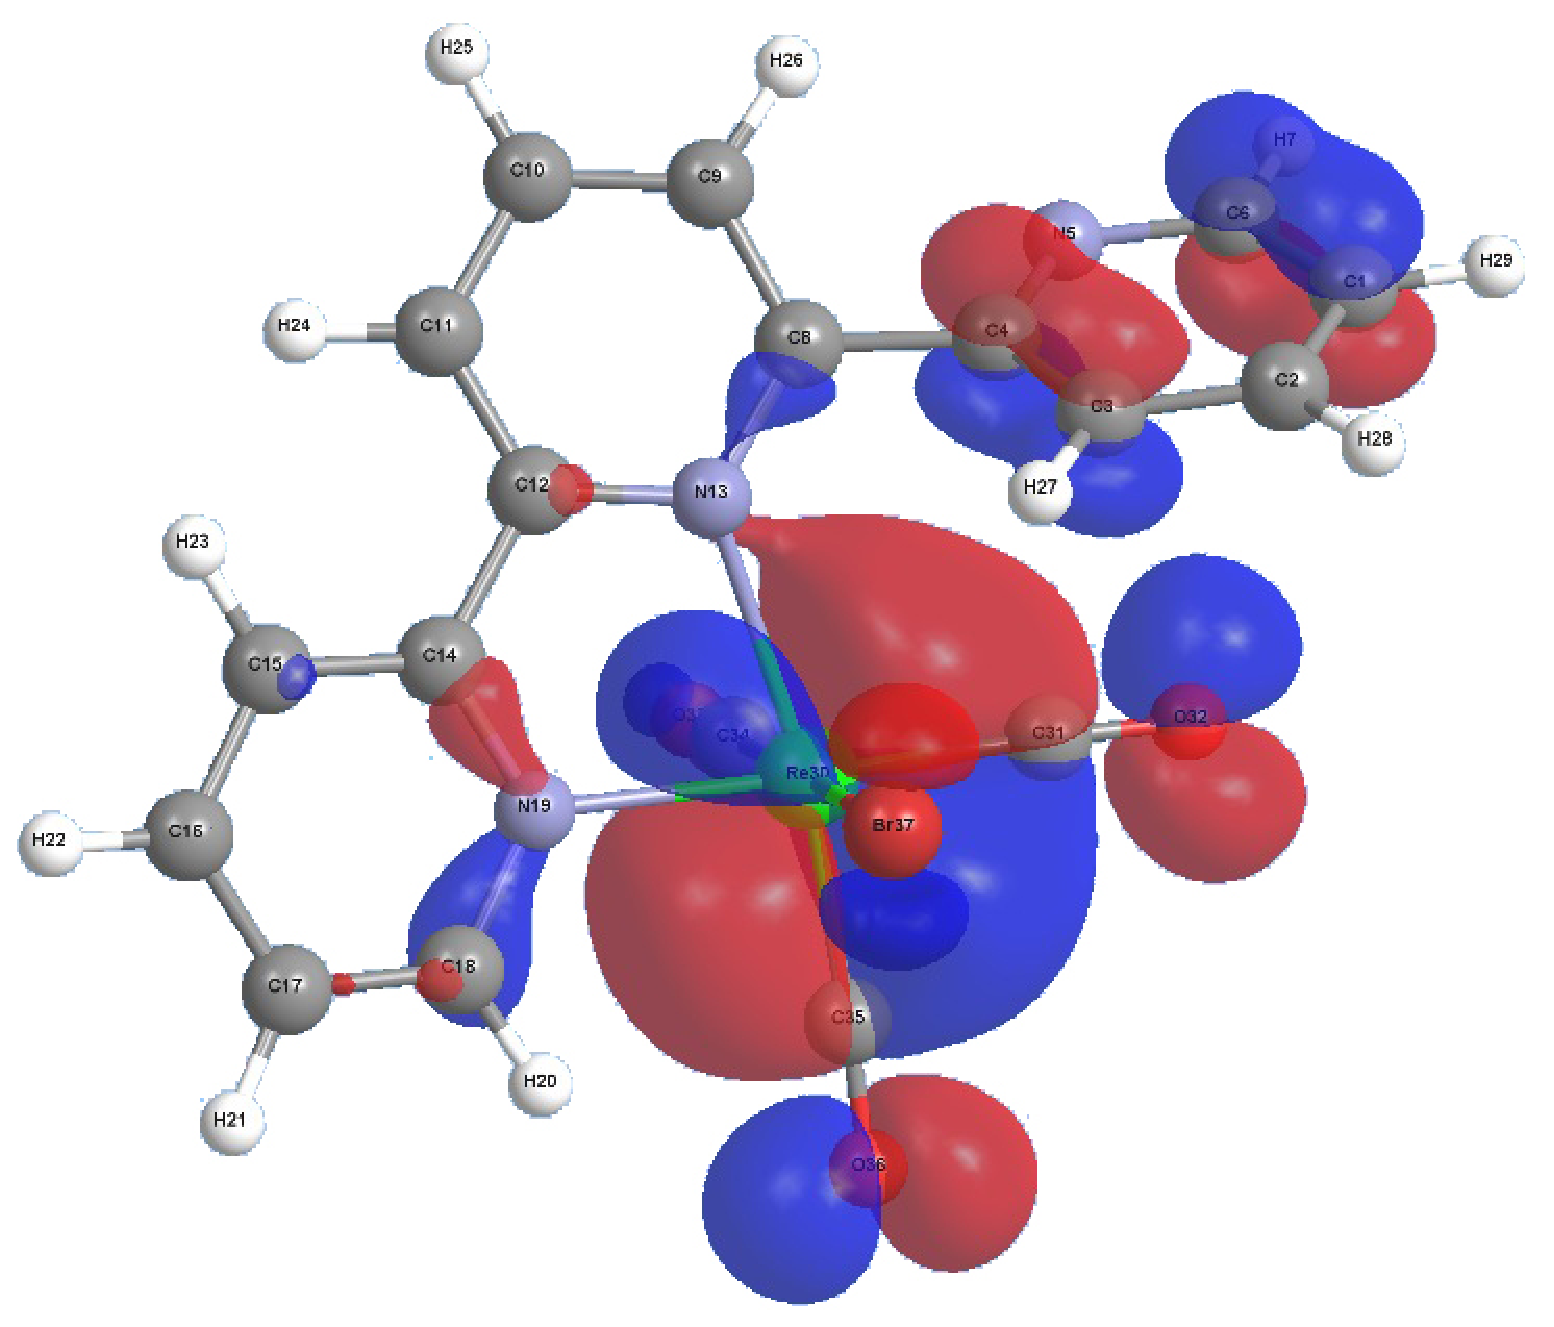
\includegraphics[clip=true, width=\textwidth, keepaspectratio]{images/mos/3h-2.eps}
  \caption{HOMO-2}
 \end{subfigure}
 \begin{subfigure}[b]{0.31\textwidth}
  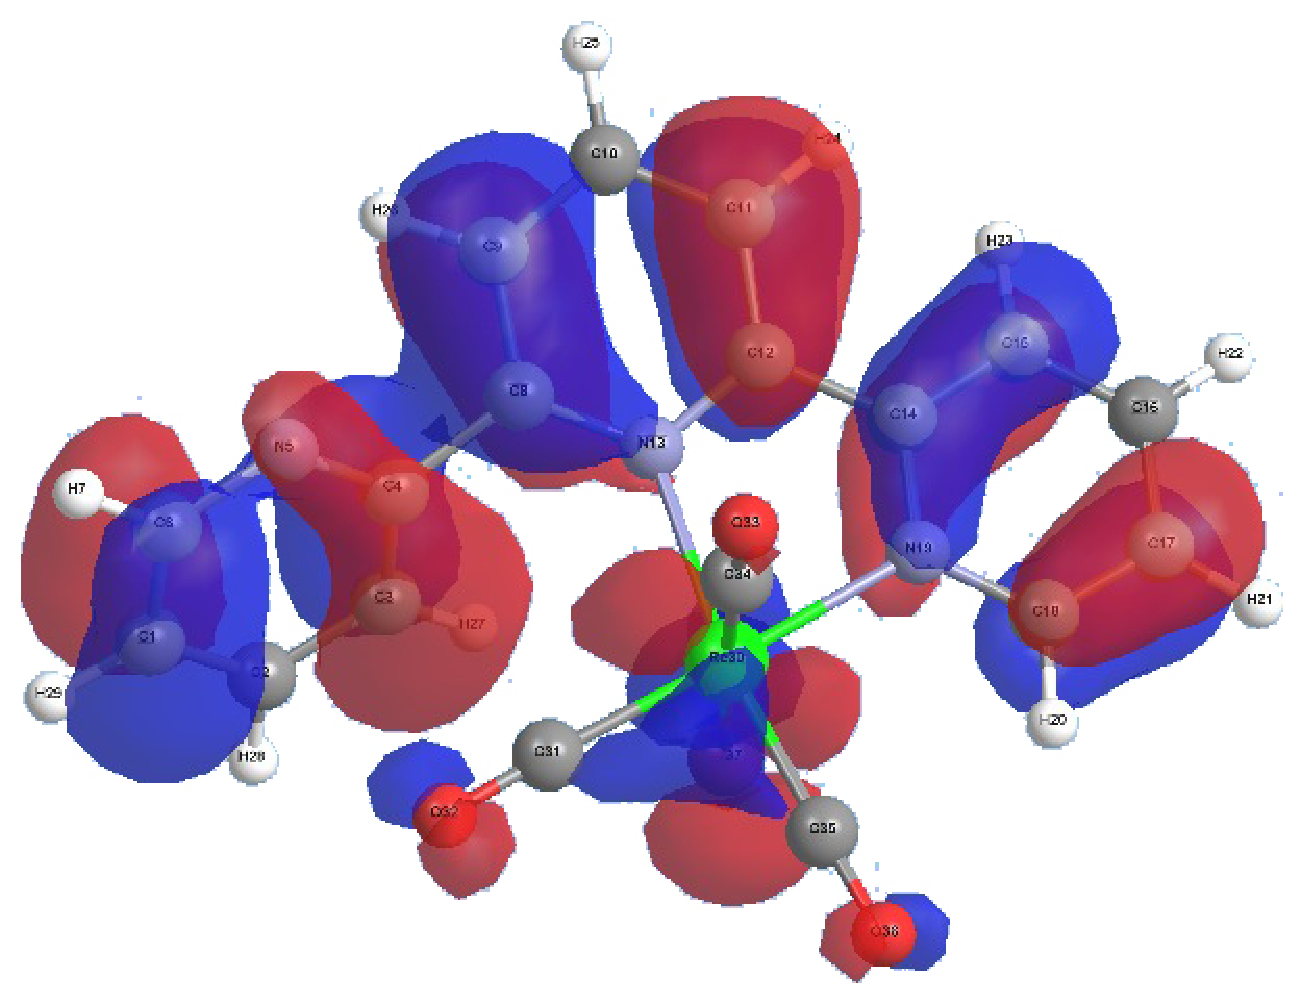
\includegraphics[clip=true, width=\textwidth, keepaspectratio]{images/mos/3h-3.eps}
  \caption{HOMO-3}
 \end{subfigure}
\caption[Molecular orbitals HOMO-3 to LUMO+2 of \textbf{2.3}]{Isosurface plots of the frontier molecular orbitals HOMO-3 to LUMO+2 of \textbf{2.3}}
\label{fig.mo23}
\end{figure} 

\begin{figure}[!ht]
 \centering
 \begin{subfigure}[b]{0.31\textwidth}
  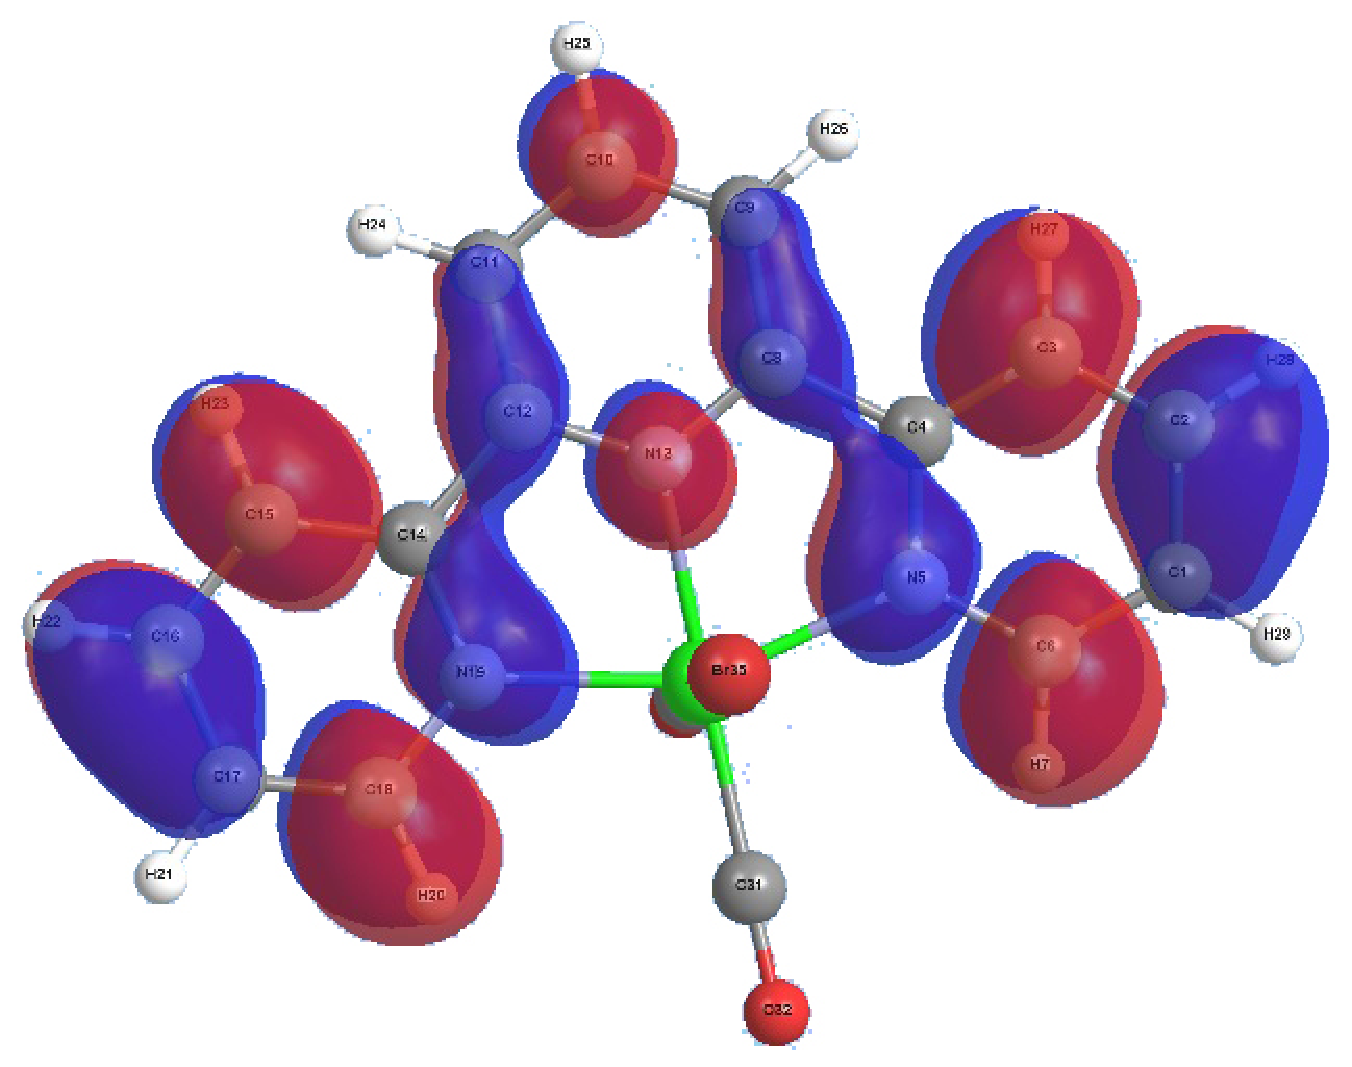
\includegraphics[clip=true, width=\textwidth, keepaspectratio]{images/mos/4l+3.eps}
  \caption{LUMO+3}
 \end{subfigure}
 \begin{subfigure}[b]{0.31\textwidth}
  \includegraphics[clip=true, width=\textwidth, keepaspectratio]{images/mos/4l+2.eps}
  \caption{LUMO+2}
 \end{subfigure}
  \begin{subfigure}[b]{0.31\textwidth}
  \includegraphics[clip=true, width=\textwidth, keepaspectratio]{images/mos/4l+1.eps}
  \caption{LUMO+1}
 \end{subfigure}
  \begin{subfigure}[b]{0.31\textwidth}
  \includegraphics[clip=true, width=\textwidth, keepaspectratio]{images/mos/4l.eps}
  \caption{LUMO}
 \end{subfigure}
 \begin{subfigure}[b]{0.31\textwidth}
  \includegraphics[clip=true, width=\textwidth, keepaspectratio]{images/mos/4h.eps}
  \caption{HOMO}
 \end{subfigure}
 \begin{subfigure}[b]{0.31\textwidth}
  \includegraphics[clip=true, width=\textwidth, keepaspectratio]{images/mos/4h-1.eps}
  \caption{HOMO-1}
 \end{subfigure}
 \begin{subfigure}[b]{0.31\textwidth}
  \includegraphics[clip=true, width=\textwidth, keepaspectratio]{images/mos/4h-2.eps}
  \caption{HOMO-2}
 \end{subfigure}
 \begin{subfigure}[b]{0.31\textwidth}
  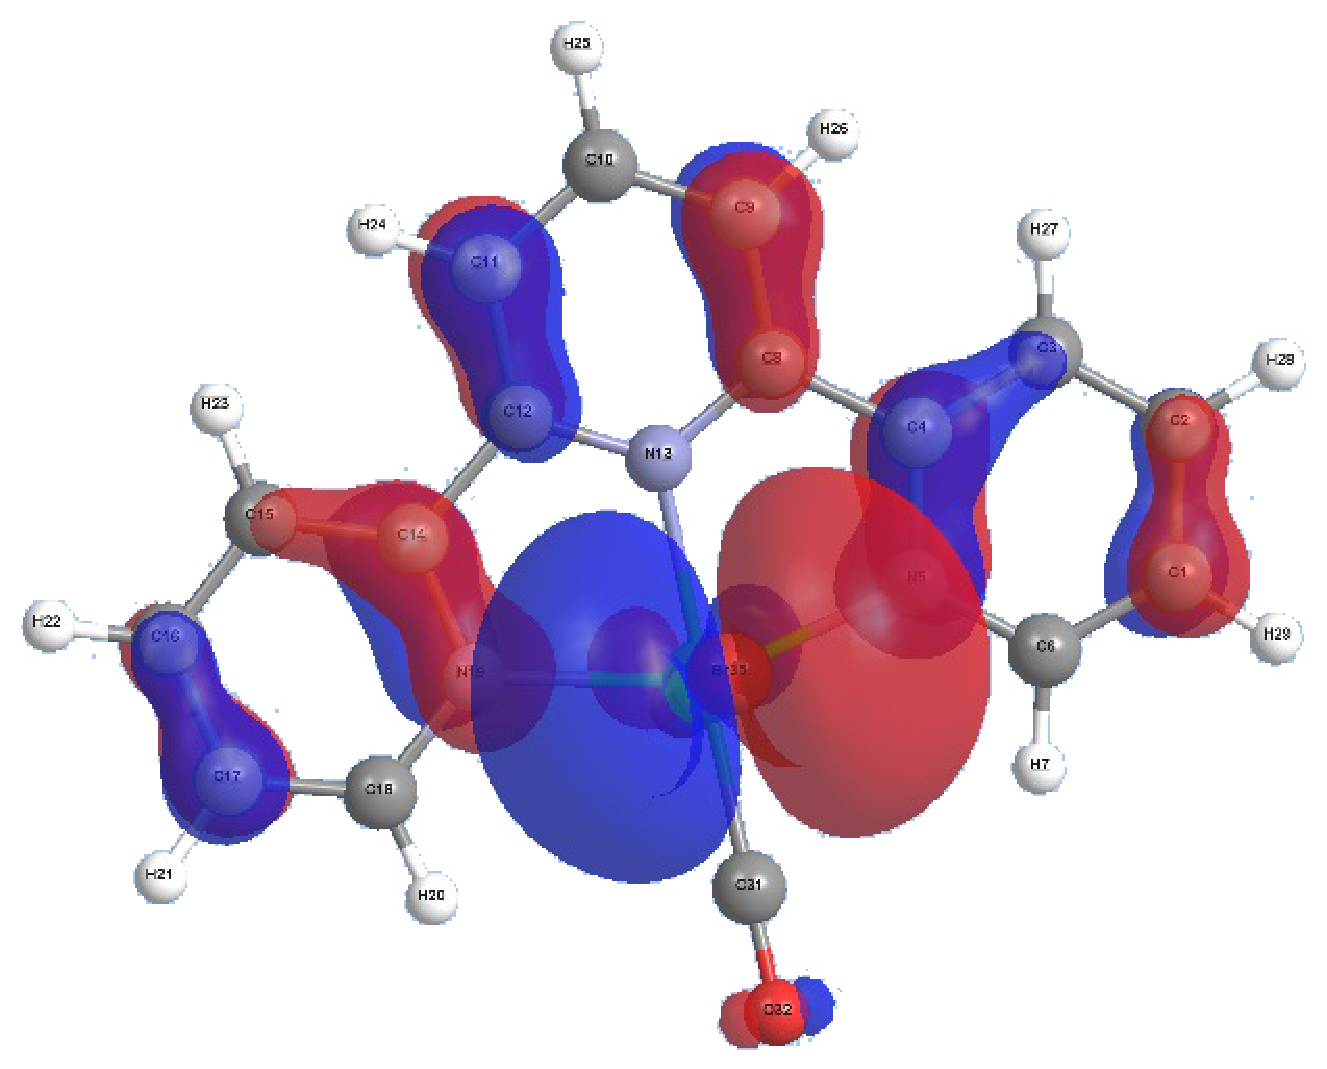
\includegraphics[clip=true, width=\textwidth, keepaspectratio]{images/mos/4h-3.eps}
  \caption{HOMO-3}
 \end{subfigure}
 \begin{subfigure}[b]{0.31\textwidth}
  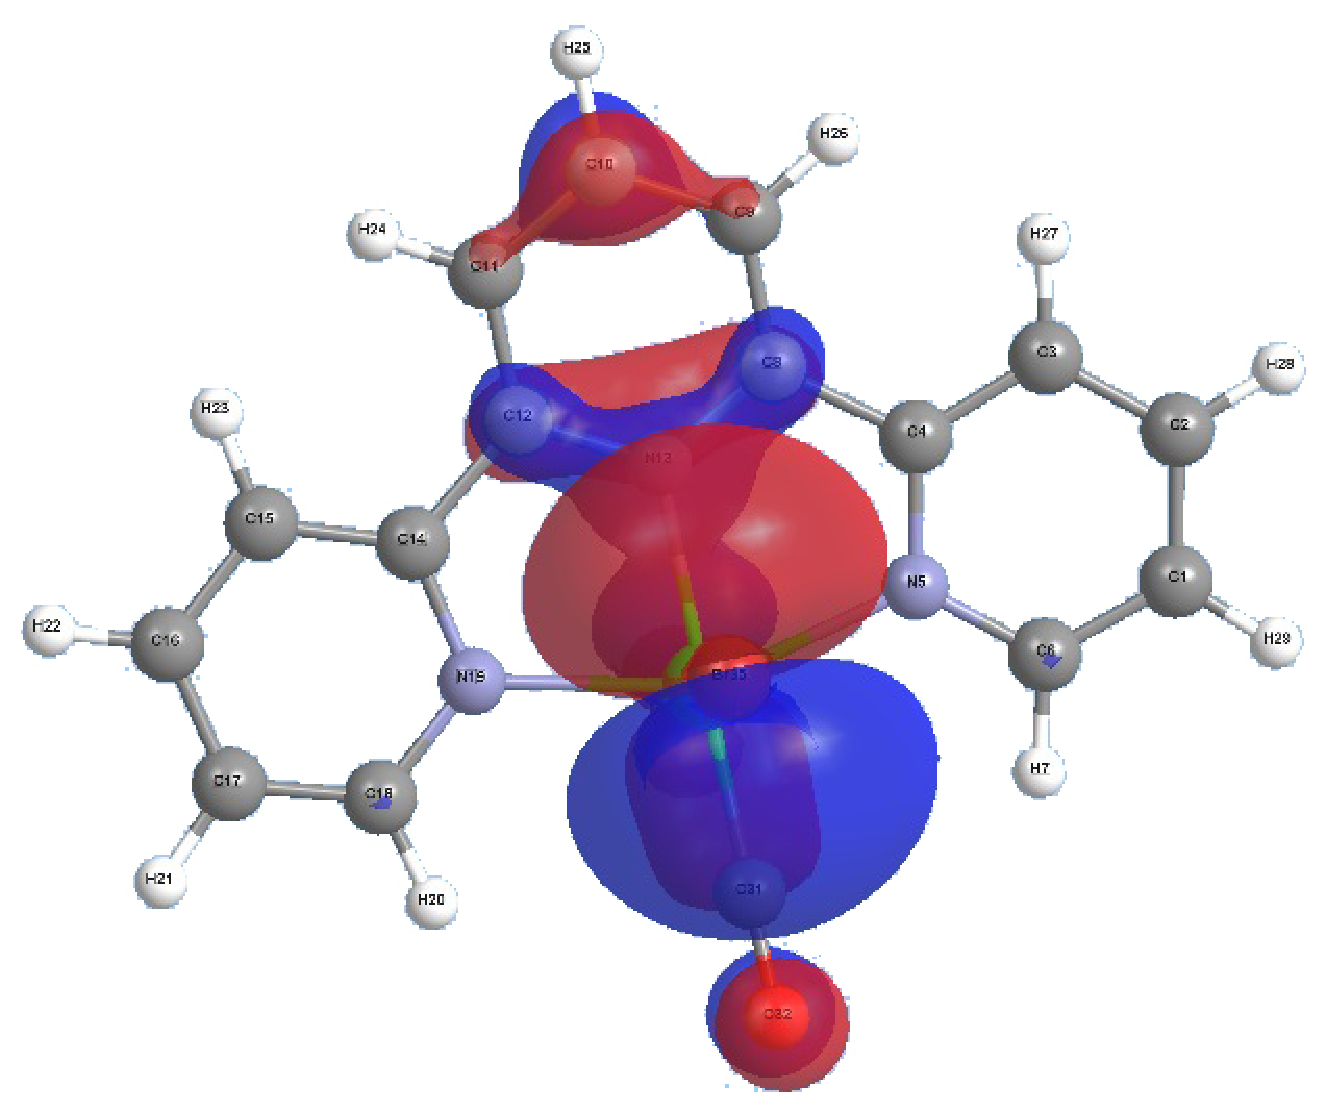
\includegraphics[clip=true, width=\textwidth, keepaspectratio]{images/mos/4h-4.eps}
  \caption{HOMO-5}
 \end{subfigure}
 \begin{subfigure}[b]{0.31\textwidth}
  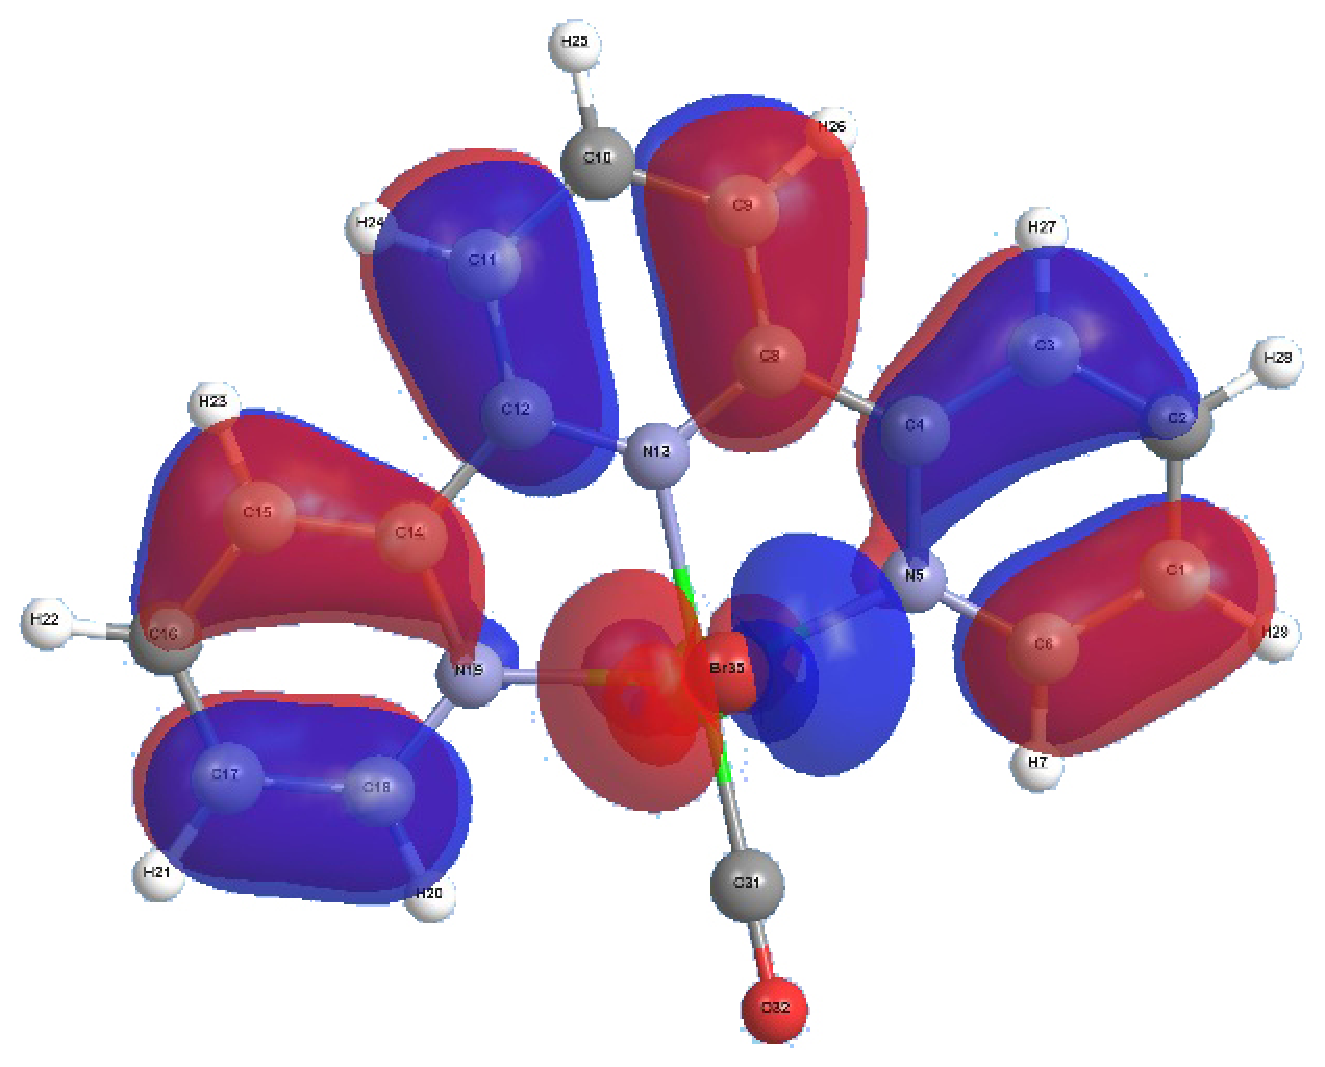
\includegraphics[clip=true, width=\textwidth, keepaspectratio]{images/mos/4h-5.eps}
  \caption{HOMO-5}
 \end{subfigure}
\caption[Molecular orbitals HOMO-5 to LUMO+3 of \textbf{2.4}]{Isosurface plots of the frontier molecular orbitals HOMO-5 to LUMO+3 of \textbf{2.4}}
\label{fig.mo24}
\end{figure}

\begin{figure}[!ht]
 \centering
 \begin{subfigure}[b]{0.31\textwidth}
  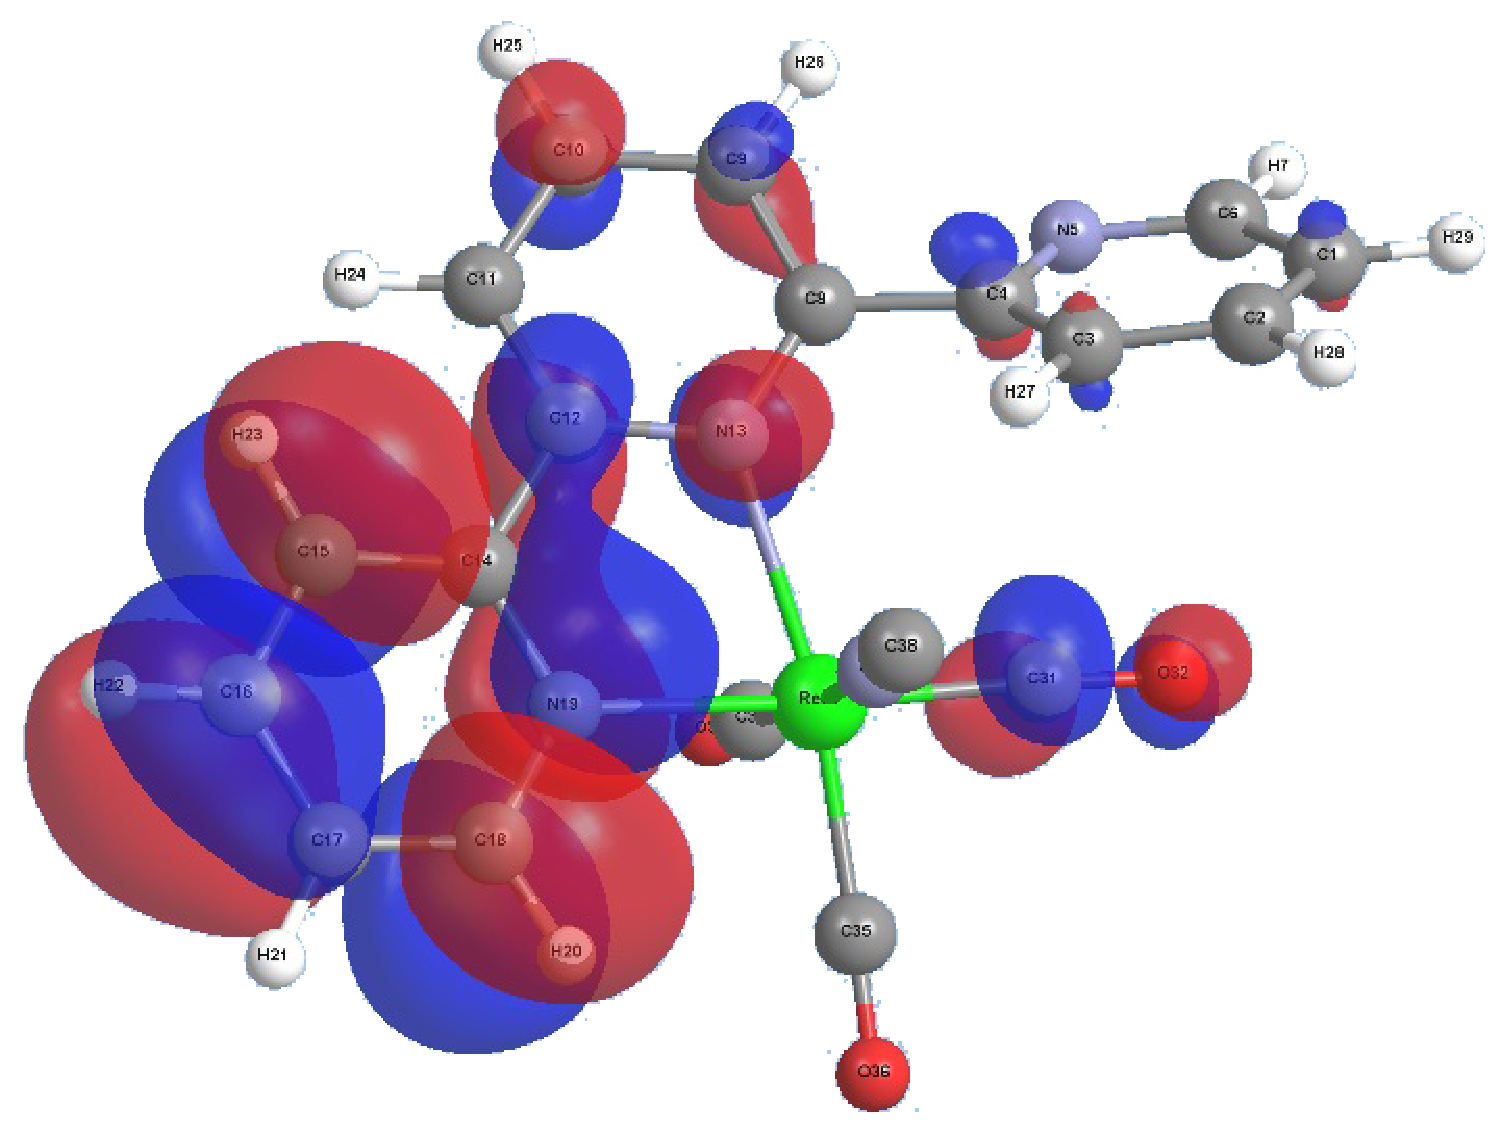
\includegraphics[clip=true, width=\textwidth, keepaspectratio]{images/mos/5l+2.eps}
  \caption{LUMO+2}
 \end{subfigure}
  \begin{subfigure}[b]{0.31\textwidth}
  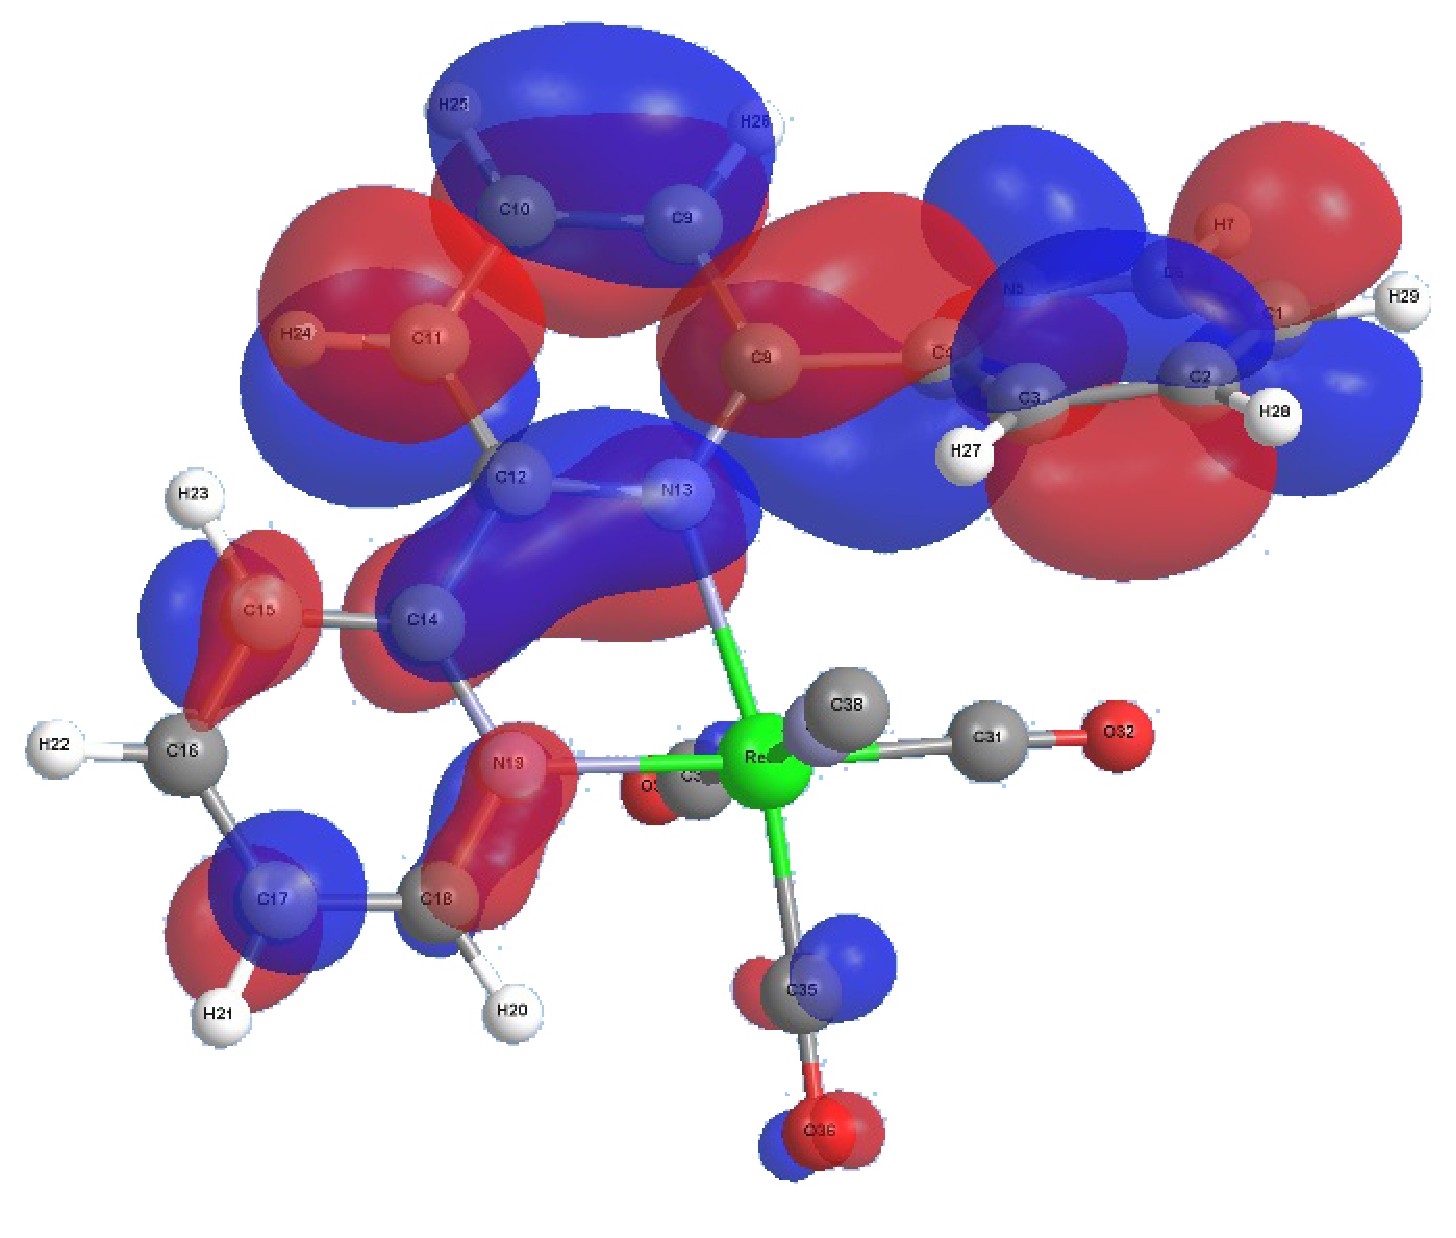
\includegraphics[clip=true, width=\textwidth, keepaspectratio]{images/mos/5l+1.eps}
  \caption{LUMO+1}
 \end{subfigure}
  \begin{subfigure}[b]{0.31\textwidth}
  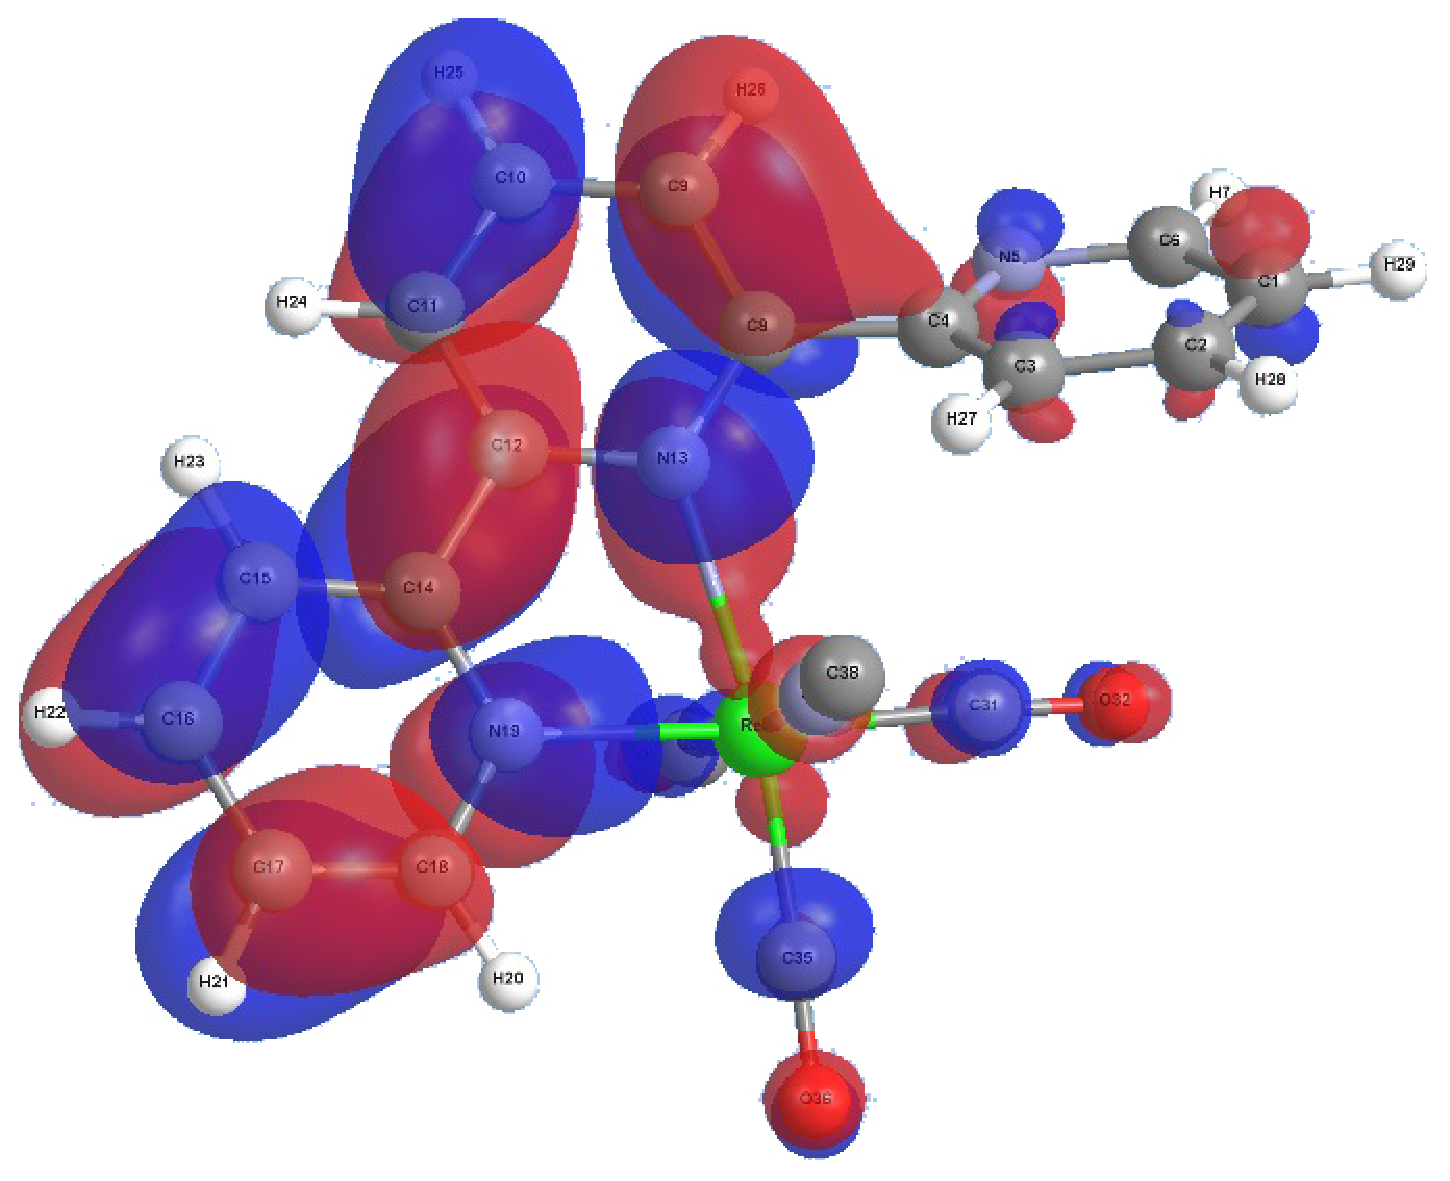
\includegraphics[clip=true, width=\textwidth, keepaspectratio]{images/mos/5l.eps}
  \caption{LUMO}
 \end{subfigure}
 \begin{subfigure}[b]{0.31\textwidth}
  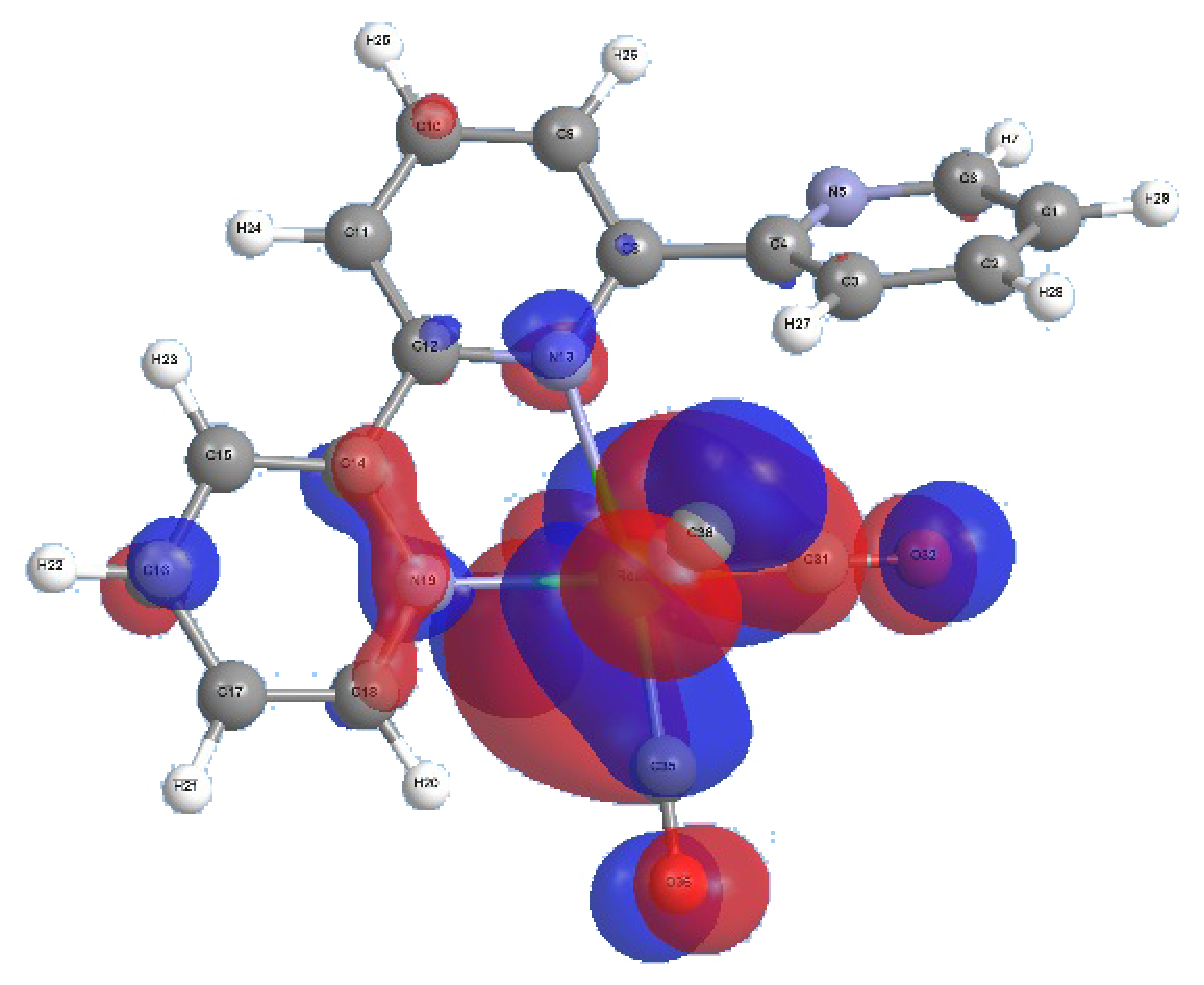
\includegraphics[clip=true, width=\textwidth, keepaspectratio]{images/mos/5h.eps}
  \caption{HOMO}
 \end{subfigure}
 \begin{subfigure}[b]{0.31\textwidth}
  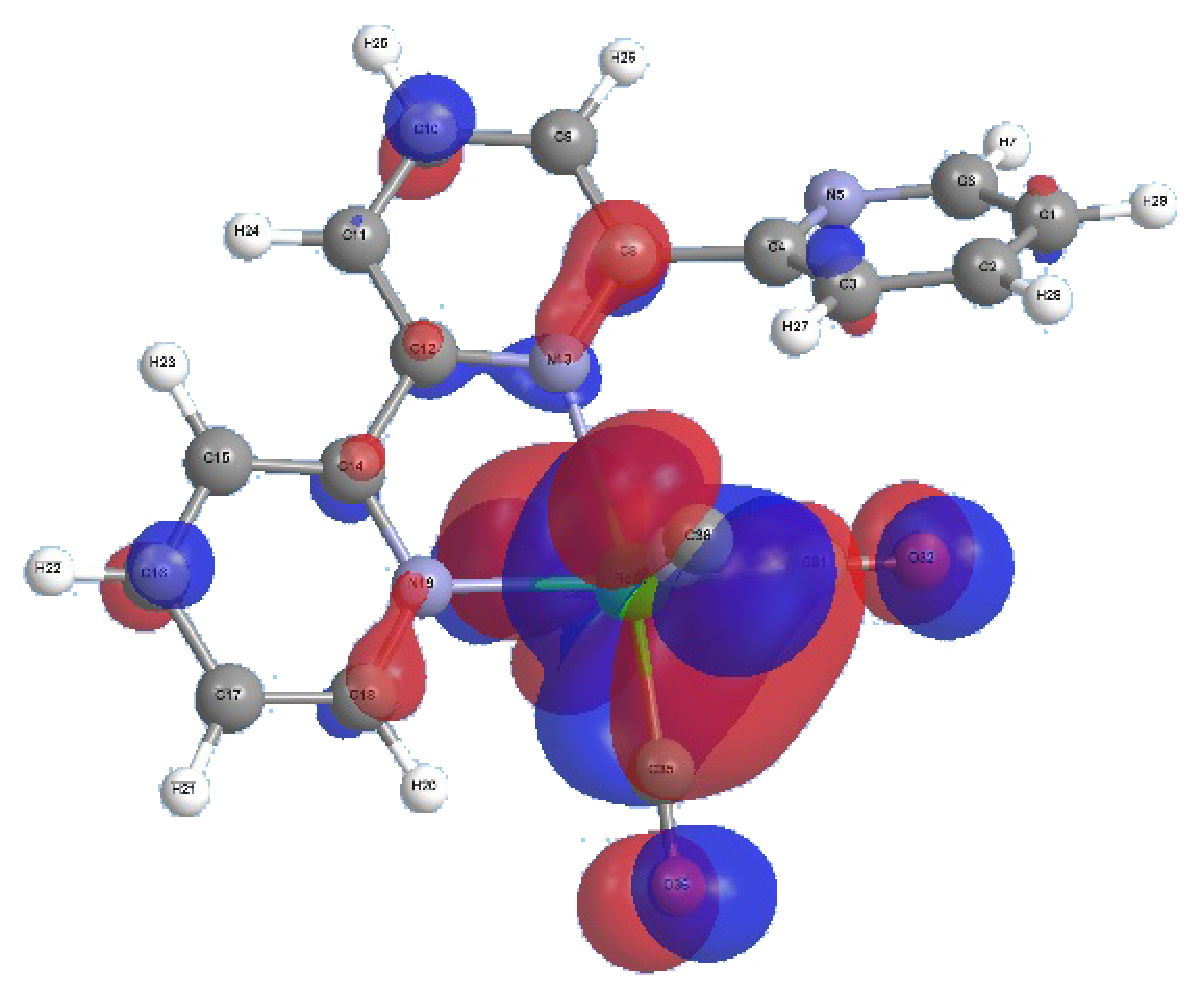
\includegraphics[clip=true, width=\textwidth, keepaspectratio]{images/mos/5h-1.eps}
  \caption{HOMO-1}
 \end{subfigure}
 \begin{subfigure}[b]{0.31\textwidth}
  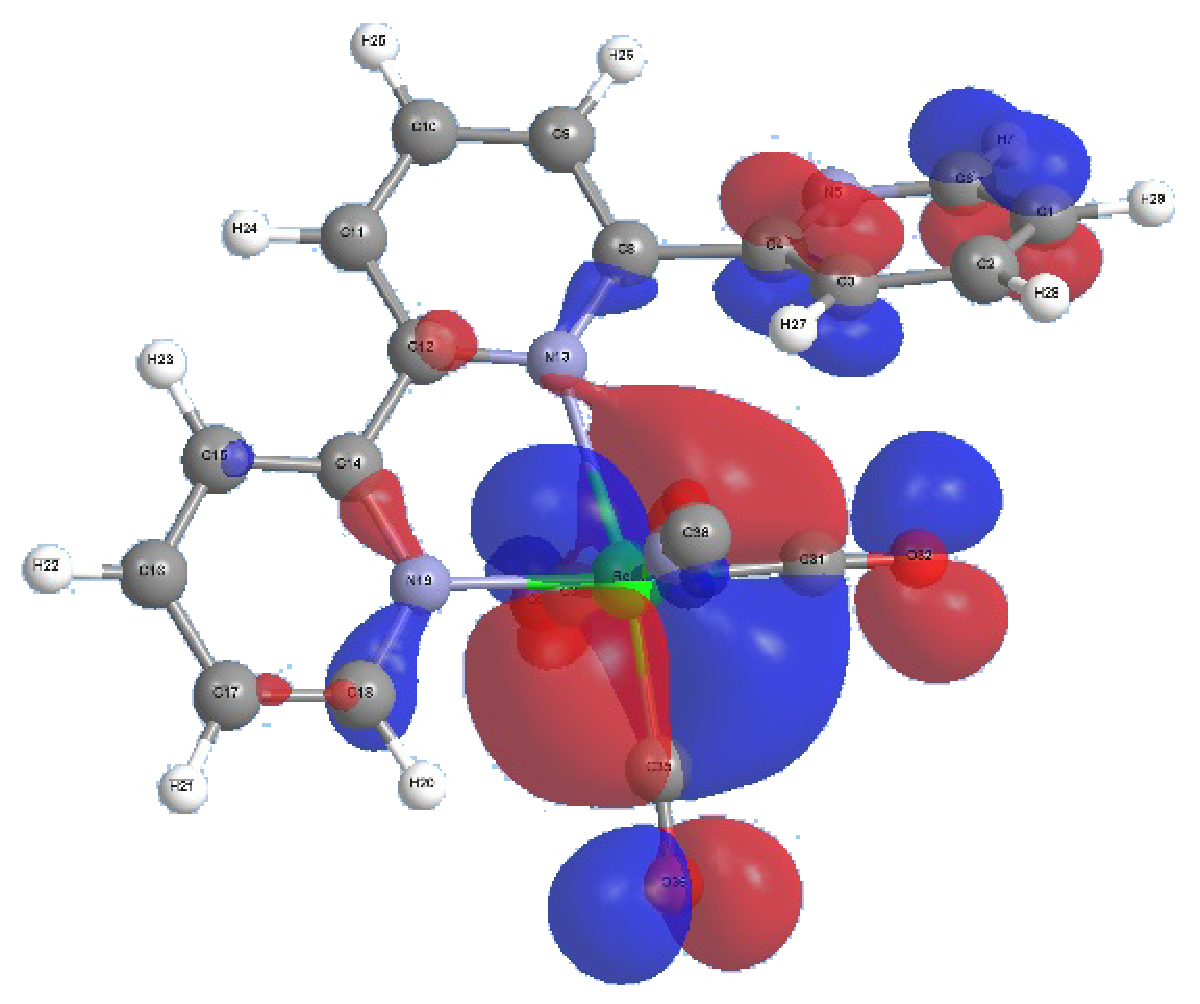
\includegraphics[clip=true, width=\textwidth, keepaspectratio]{images/mos/5h-2.eps}
  \caption{HOMO-2}
 \end{subfigure}
 \begin{subfigure}[b]{0.31\textwidth}
  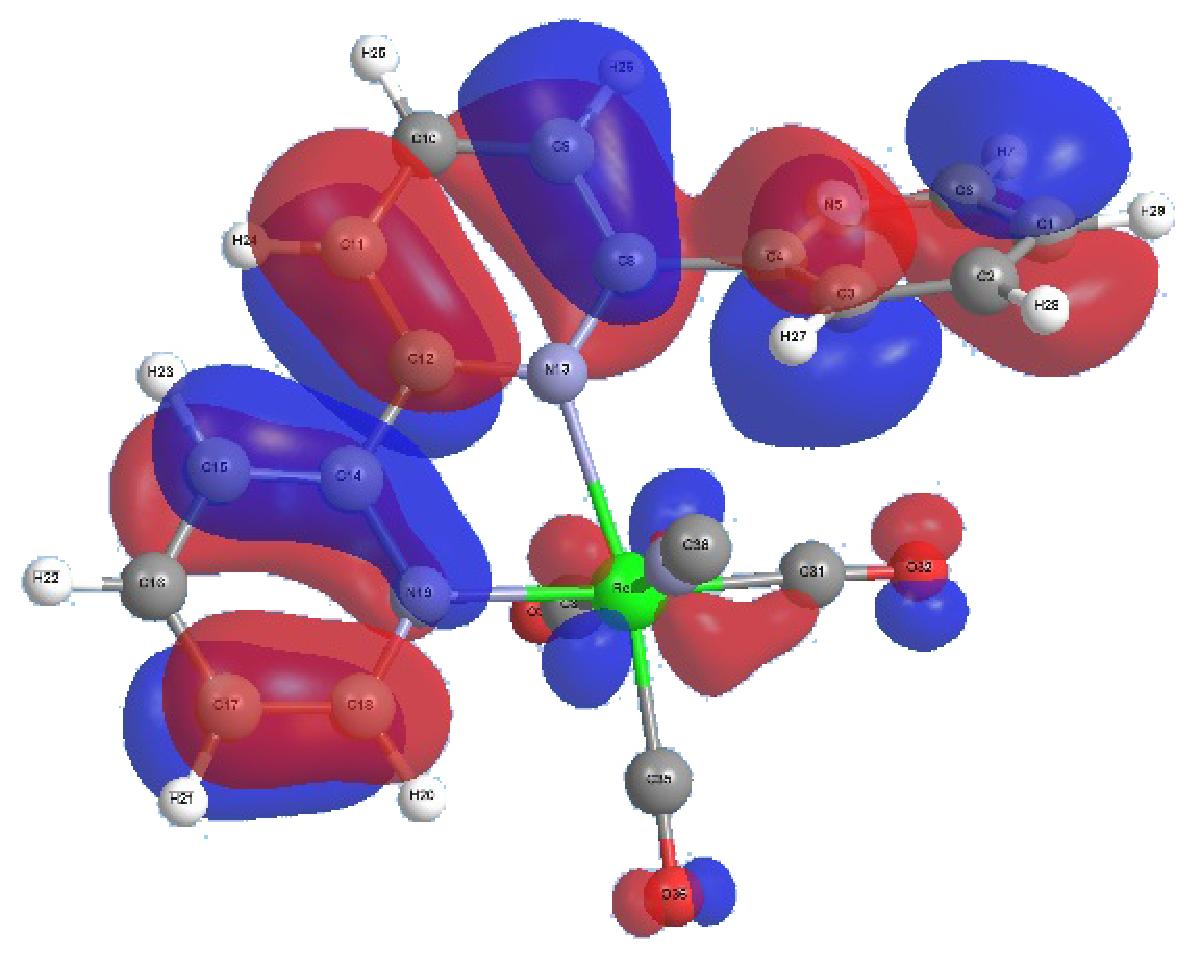
\includegraphics[clip=true, width=\textwidth, keepaspectratio]{images/mos/5h-3.eps}
  \caption{HOMO-3}
 \end{subfigure}
\caption[Molecular orbitals HOMO-3 to LUMO+2 of \textbf{2.5}]{Isosurface plots of the frontier molecular orbitals HOMO-3 to LUMO+2 of \textbf{2.5}}
\label{fig.mo25}
\end{figure} 

\begin{figure}[!ht]
 \centering
 \begin{subfigure}[b]{0.31\textwidth}
  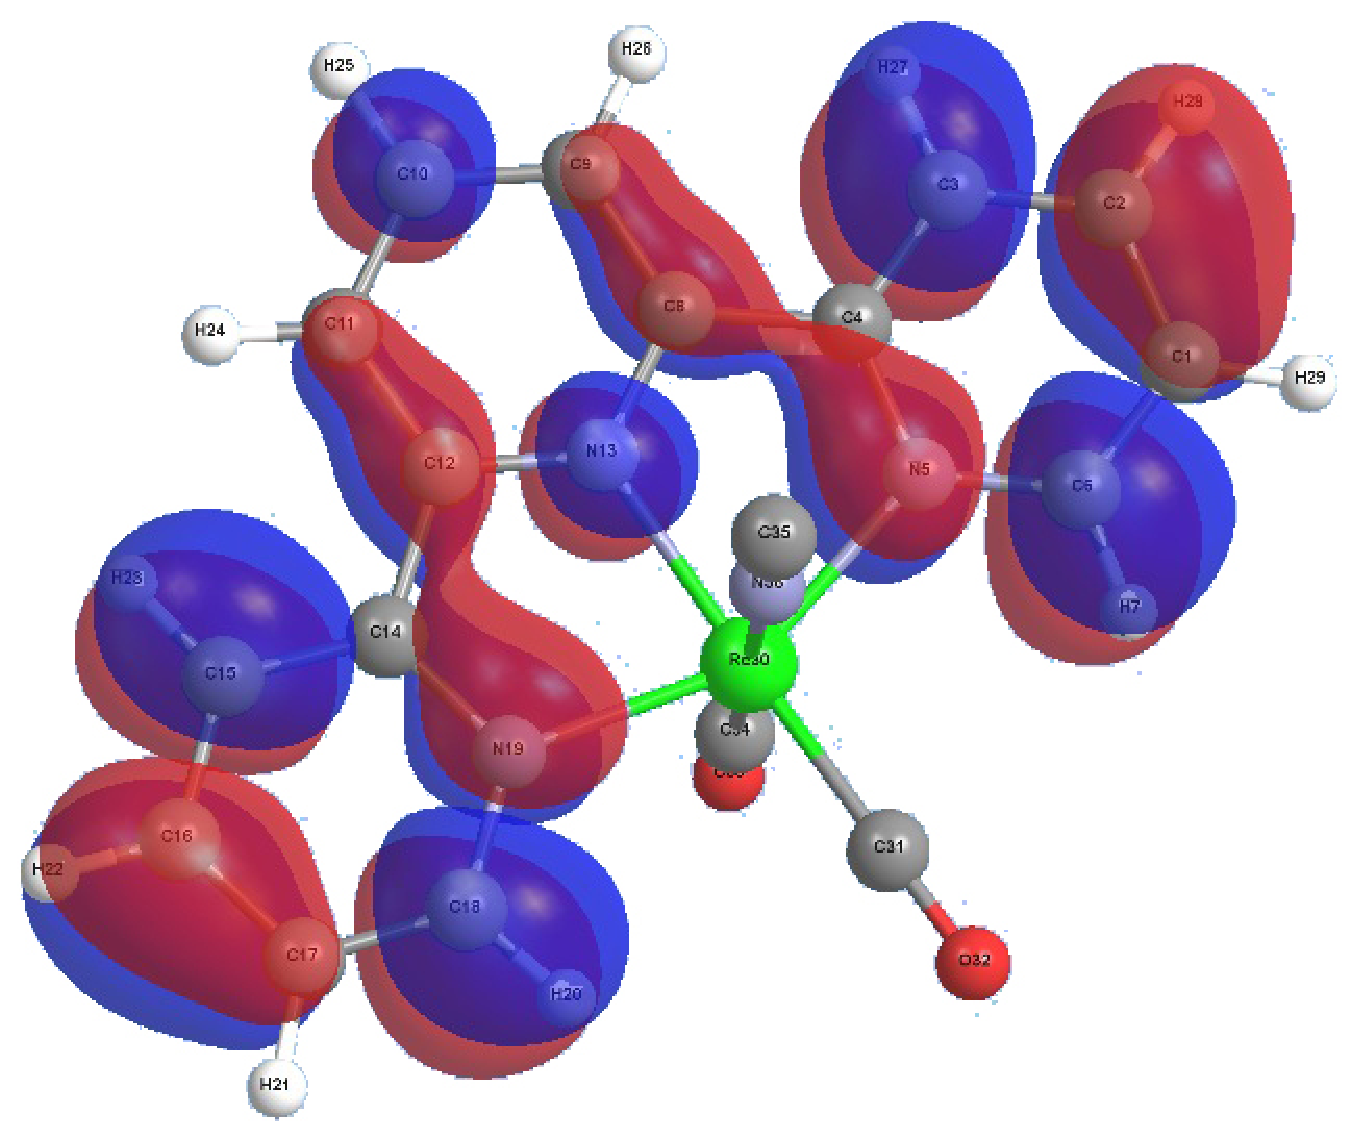
\includegraphics[clip=true, width=\textwidth, keepaspectratio]{images/mos/6l+3.eps}
  \caption{LUMO+3}
 \end{subfigure}
 \begin{subfigure}[b]{0.31\textwidth}
  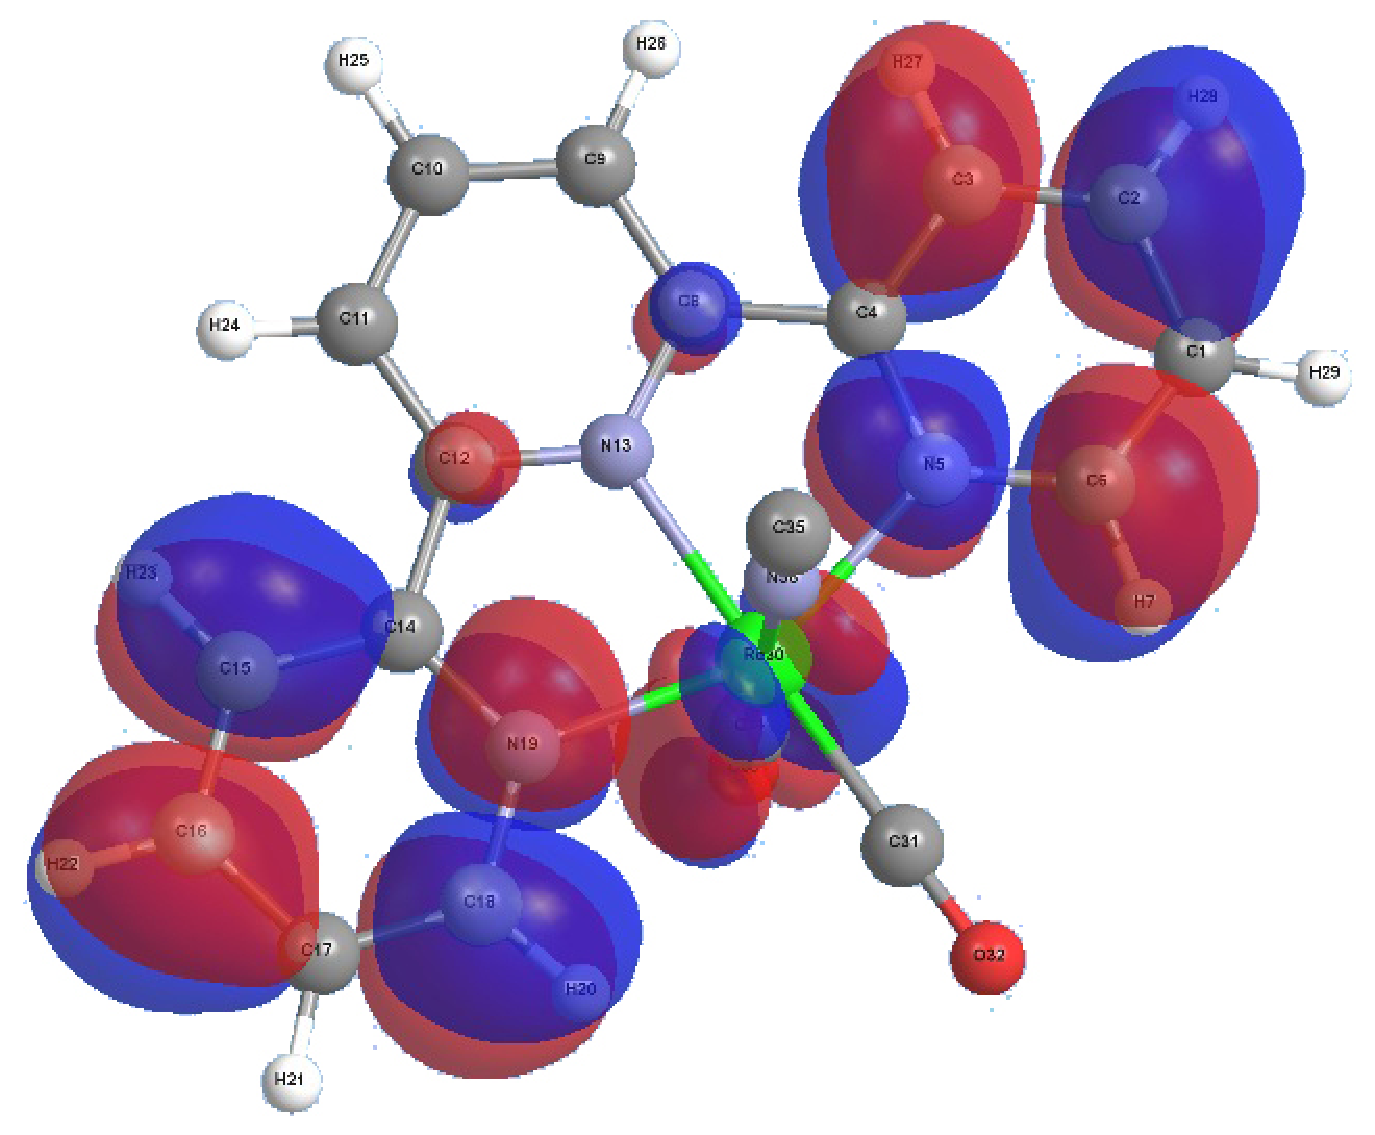
\includegraphics[clip=true, width=\textwidth, keepaspectratio]{images/mos/6l+2.eps}
  \caption{LUMO+2}
 \end{subfigure}
  \begin{subfigure}[b]{0.31\textwidth}
  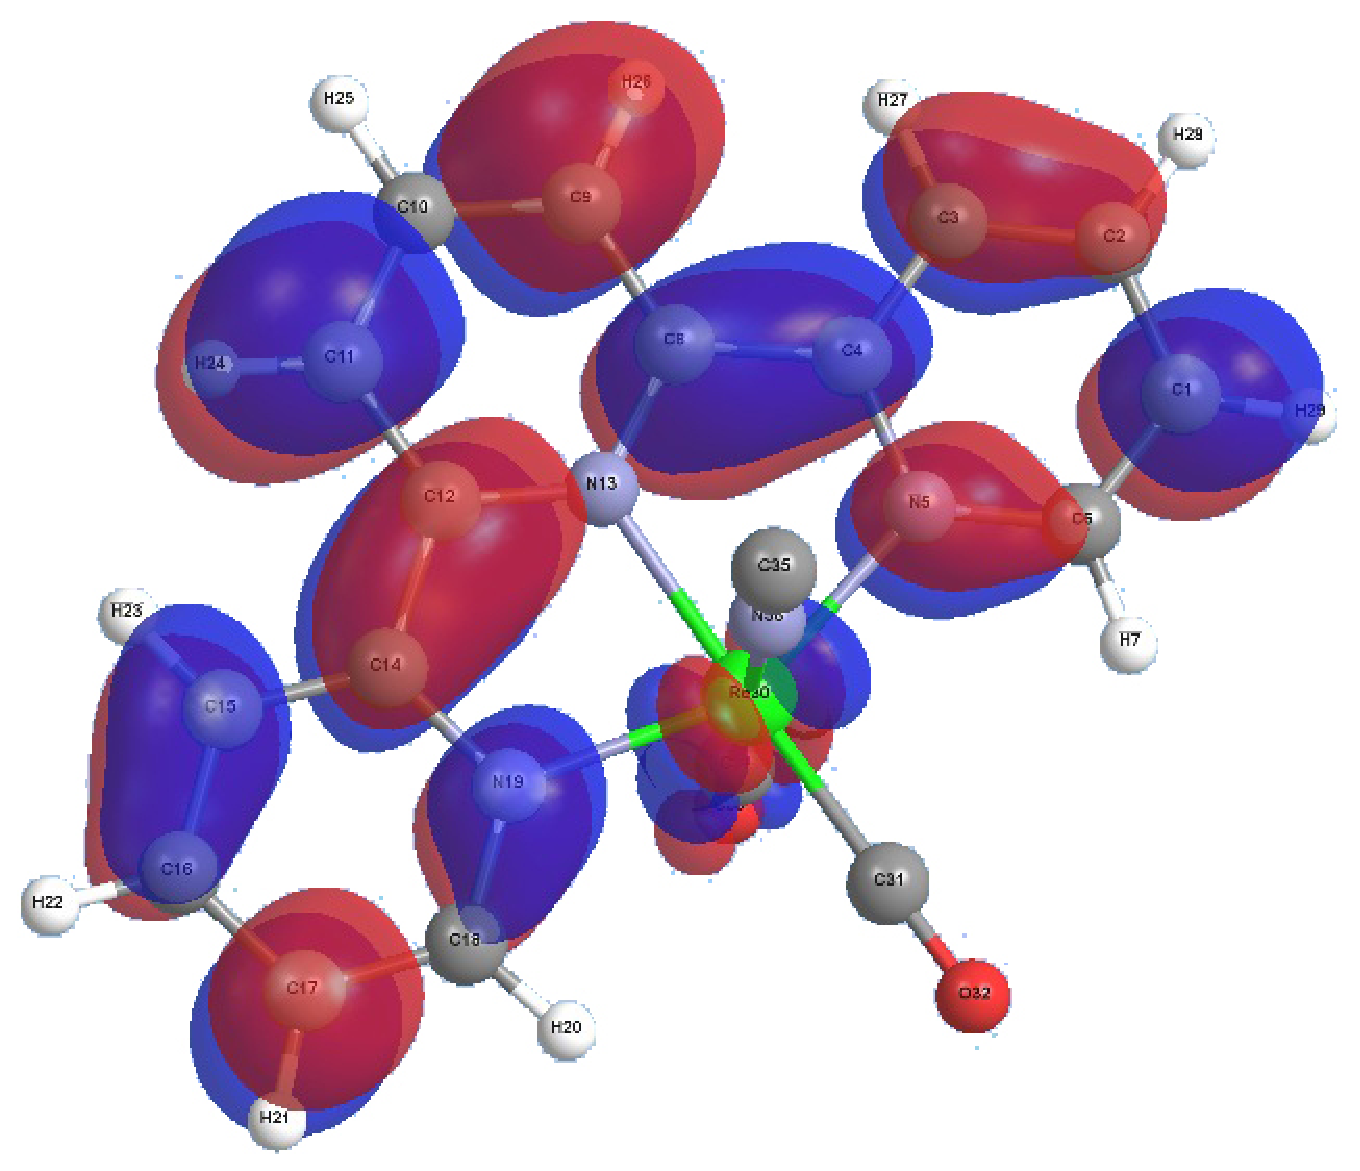
\includegraphics[clip=true, width=\textwidth, keepaspectratio]{images/mos/6l+1.eps}
  \caption{LUMO+1}
 \end{subfigure}
  \begin{subfigure}[b]{0.31\textwidth}
  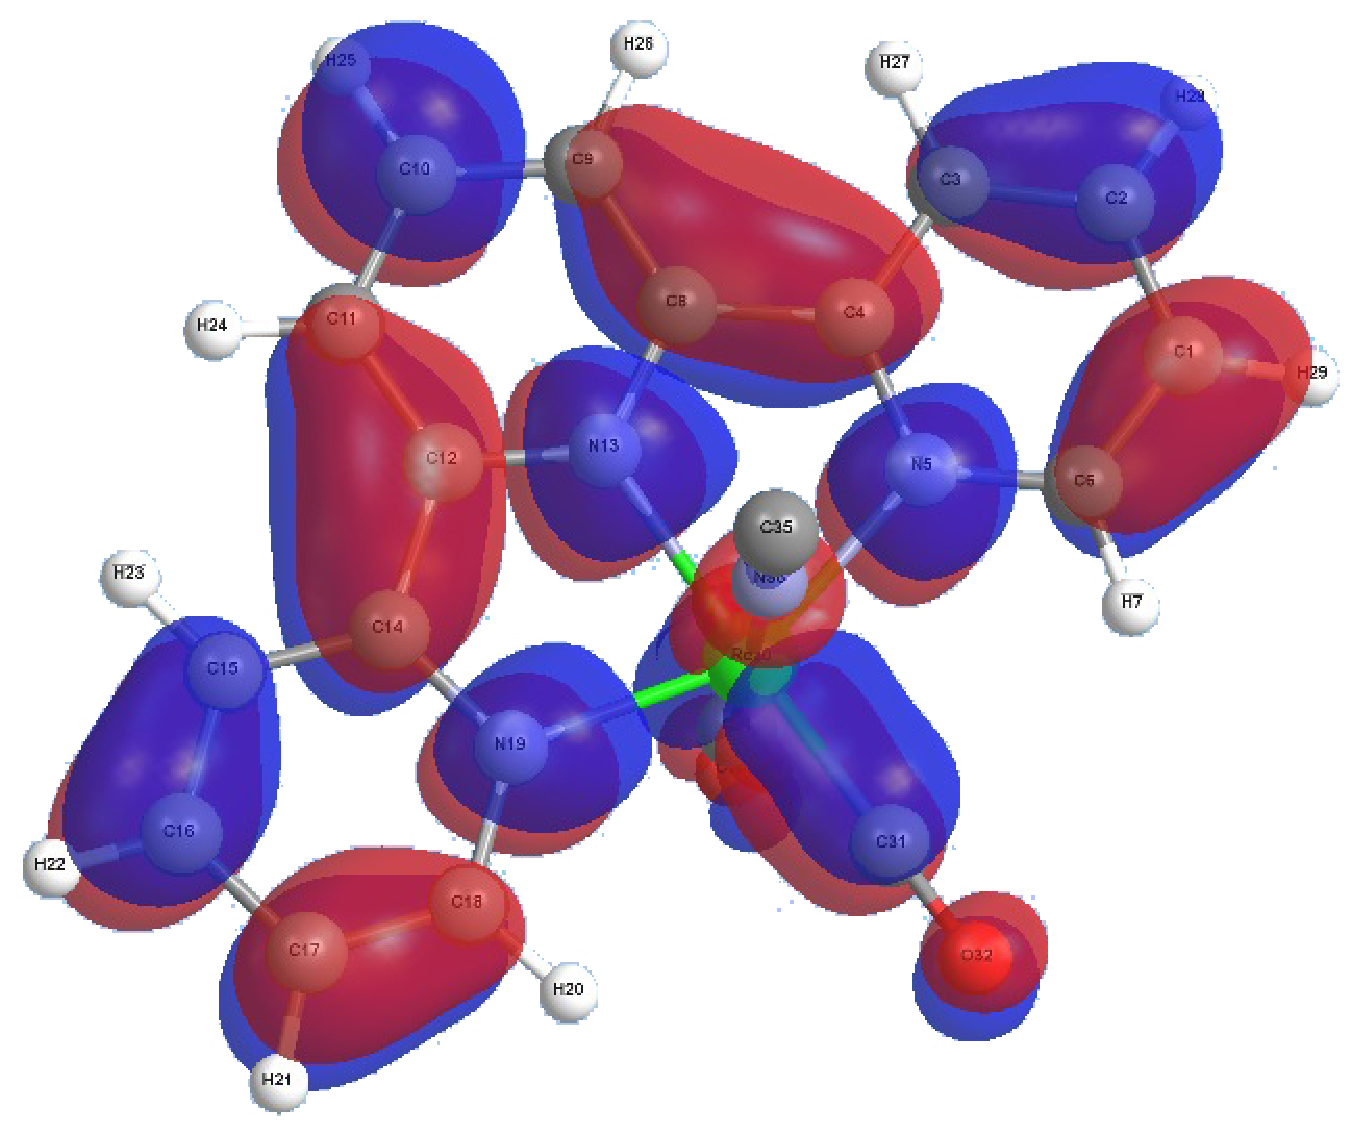
\includegraphics[clip=true, width=\textwidth, keepaspectratio]{images/mos/6l.eps}
  \caption{LUMO}
 \end{subfigure}
 \begin{subfigure}[b]{0.31\textwidth}
  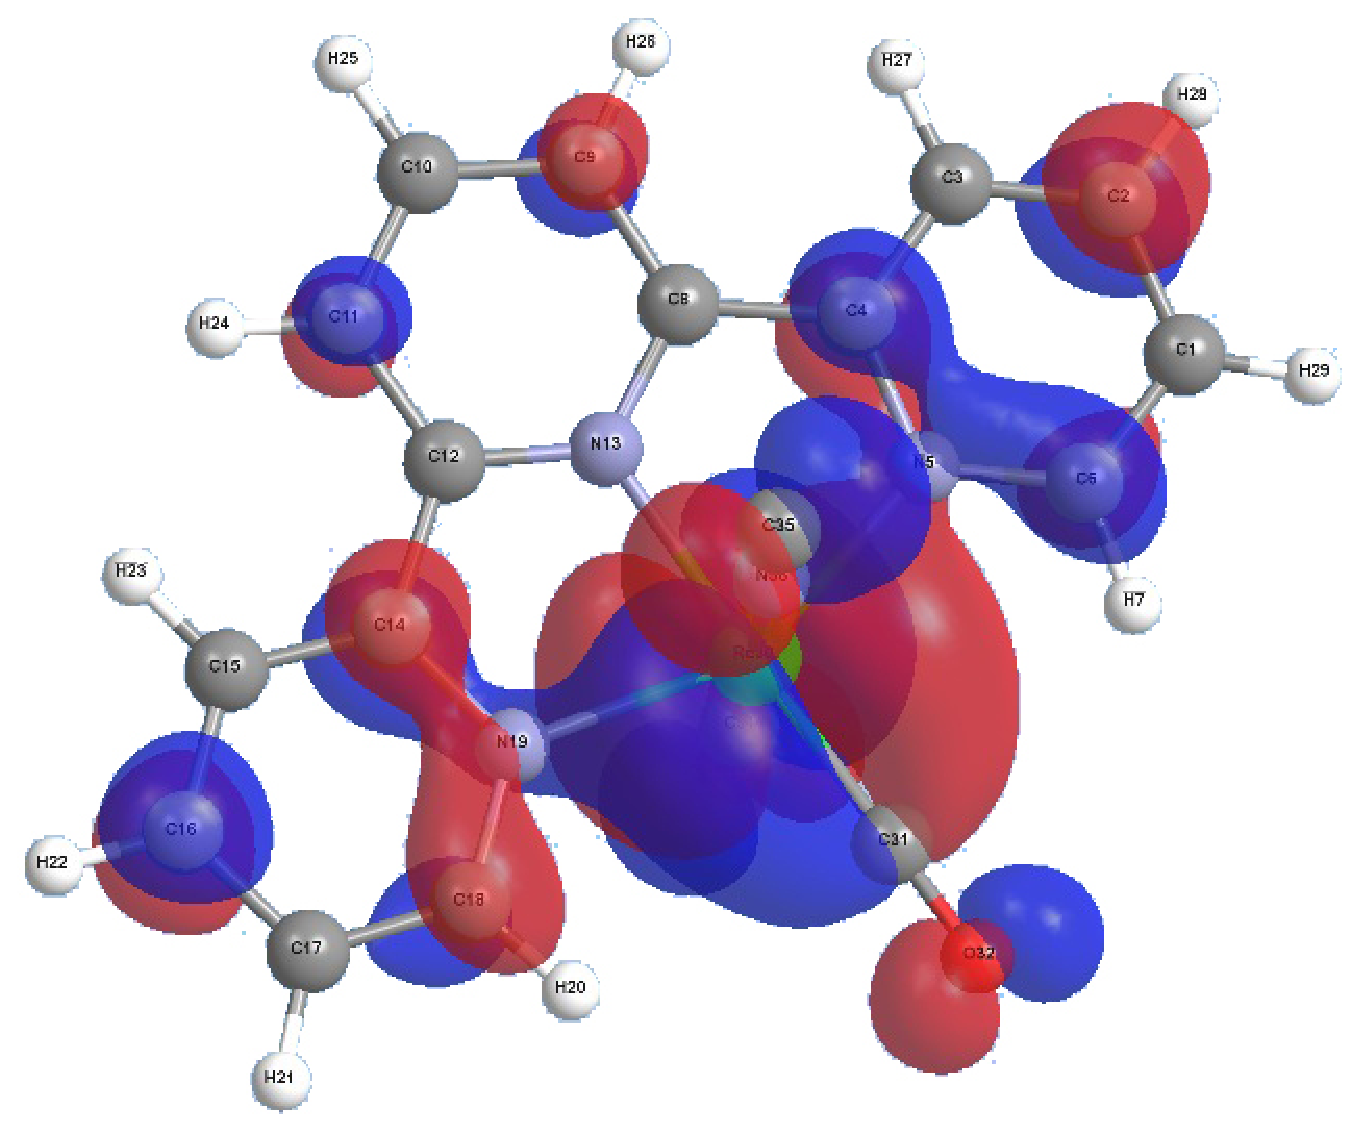
\includegraphics[clip=true, width=\textwidth, keepaspectratio]{images/mos/6h.eps}
  \caption{HOMO}
 \end{subfigure}
 \begin{subfigure}[b]{0.31\textwidth}
  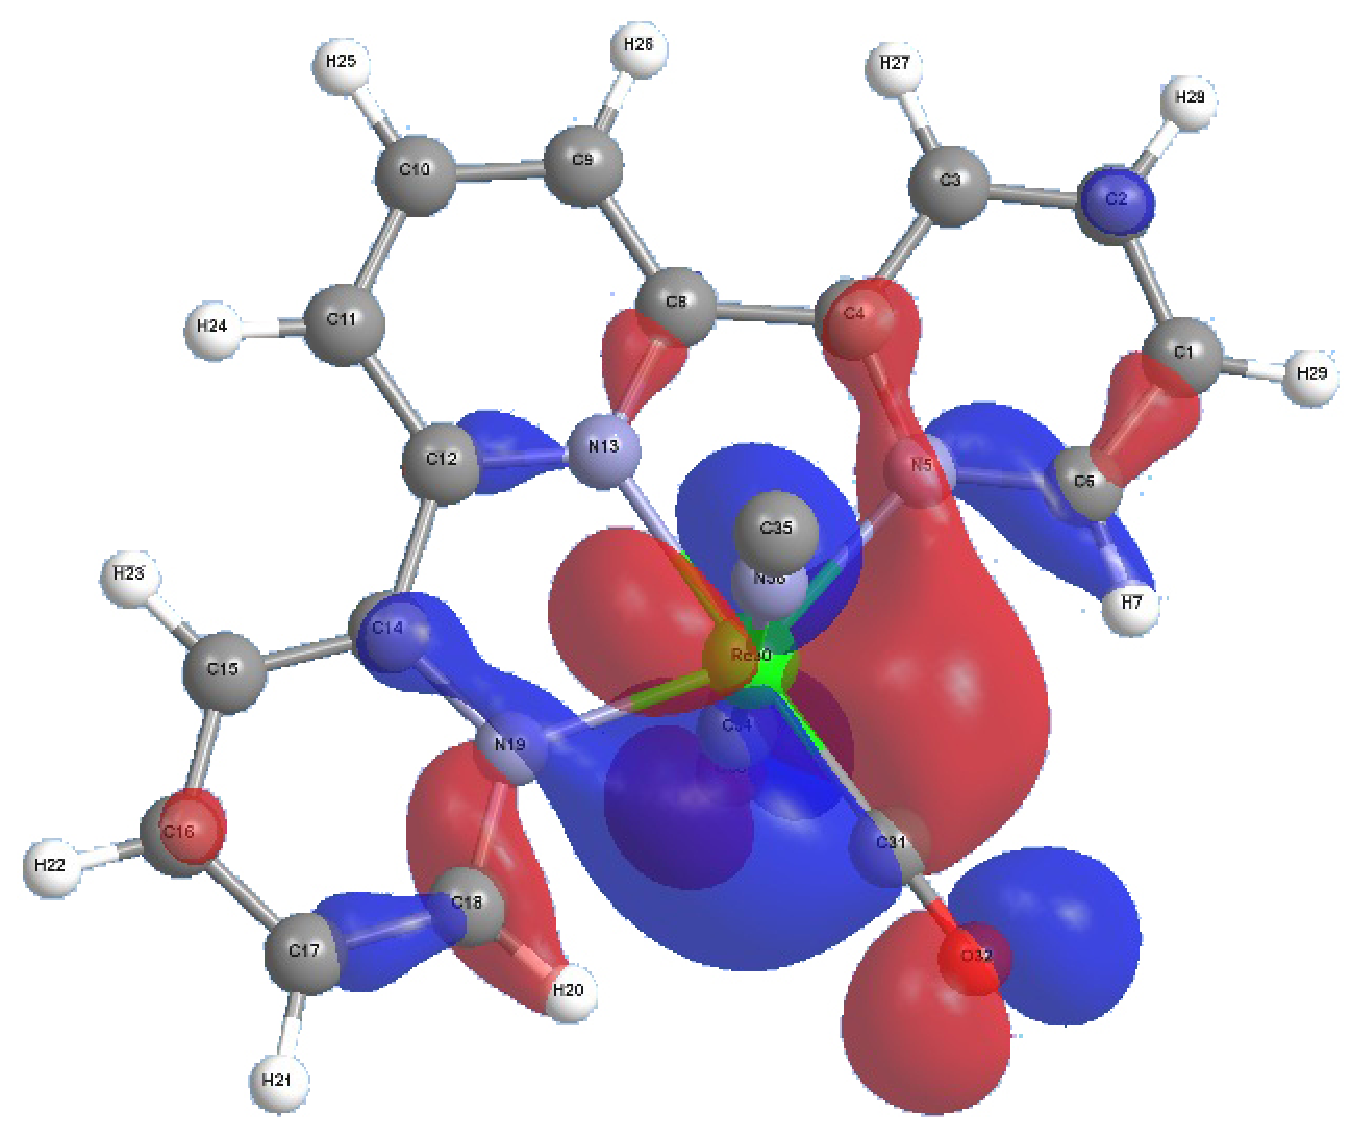
\includegraphics[clip=true, width=\textwidth, keepaspectratio]{images/mos/6h-1.eps}
  \caption{HOMO-1}
 \end{subfigure}
 \begin{subfigure}[b]{0.31\textwidth}
  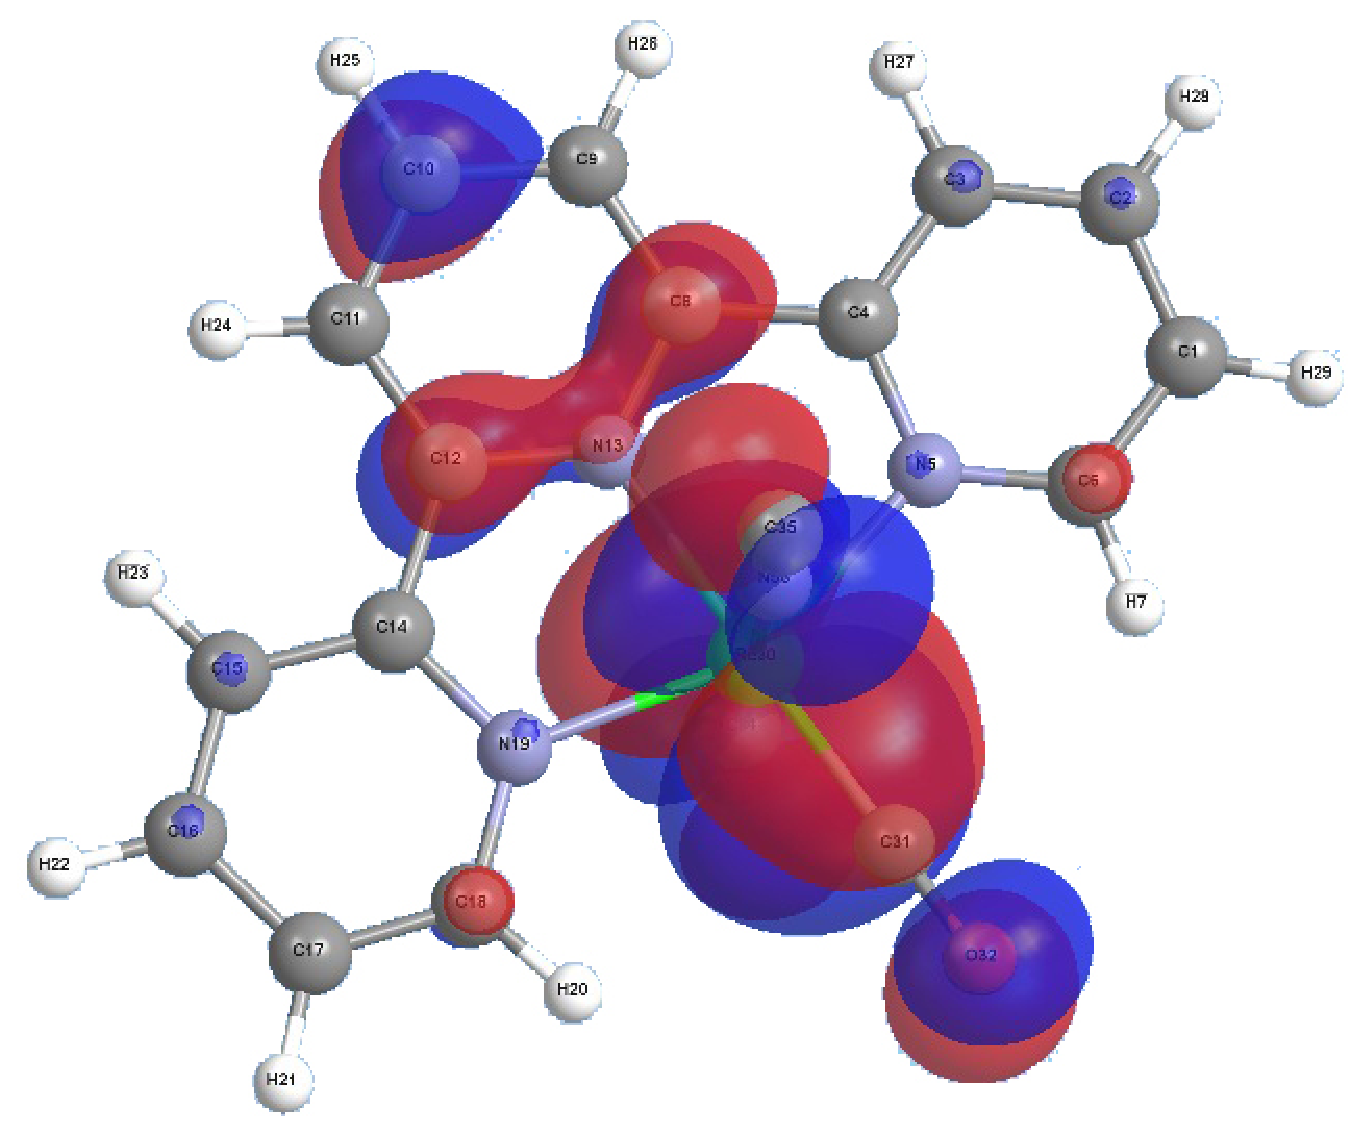
\includegraphics[clip=true, width=\textwidth, keepaspectratio]{images/mos/6h-2.eps}
  \caption{HOMO-2}
 \end{subfigure}
 \begin{subfigure}[b]{0.31\textwidth}
  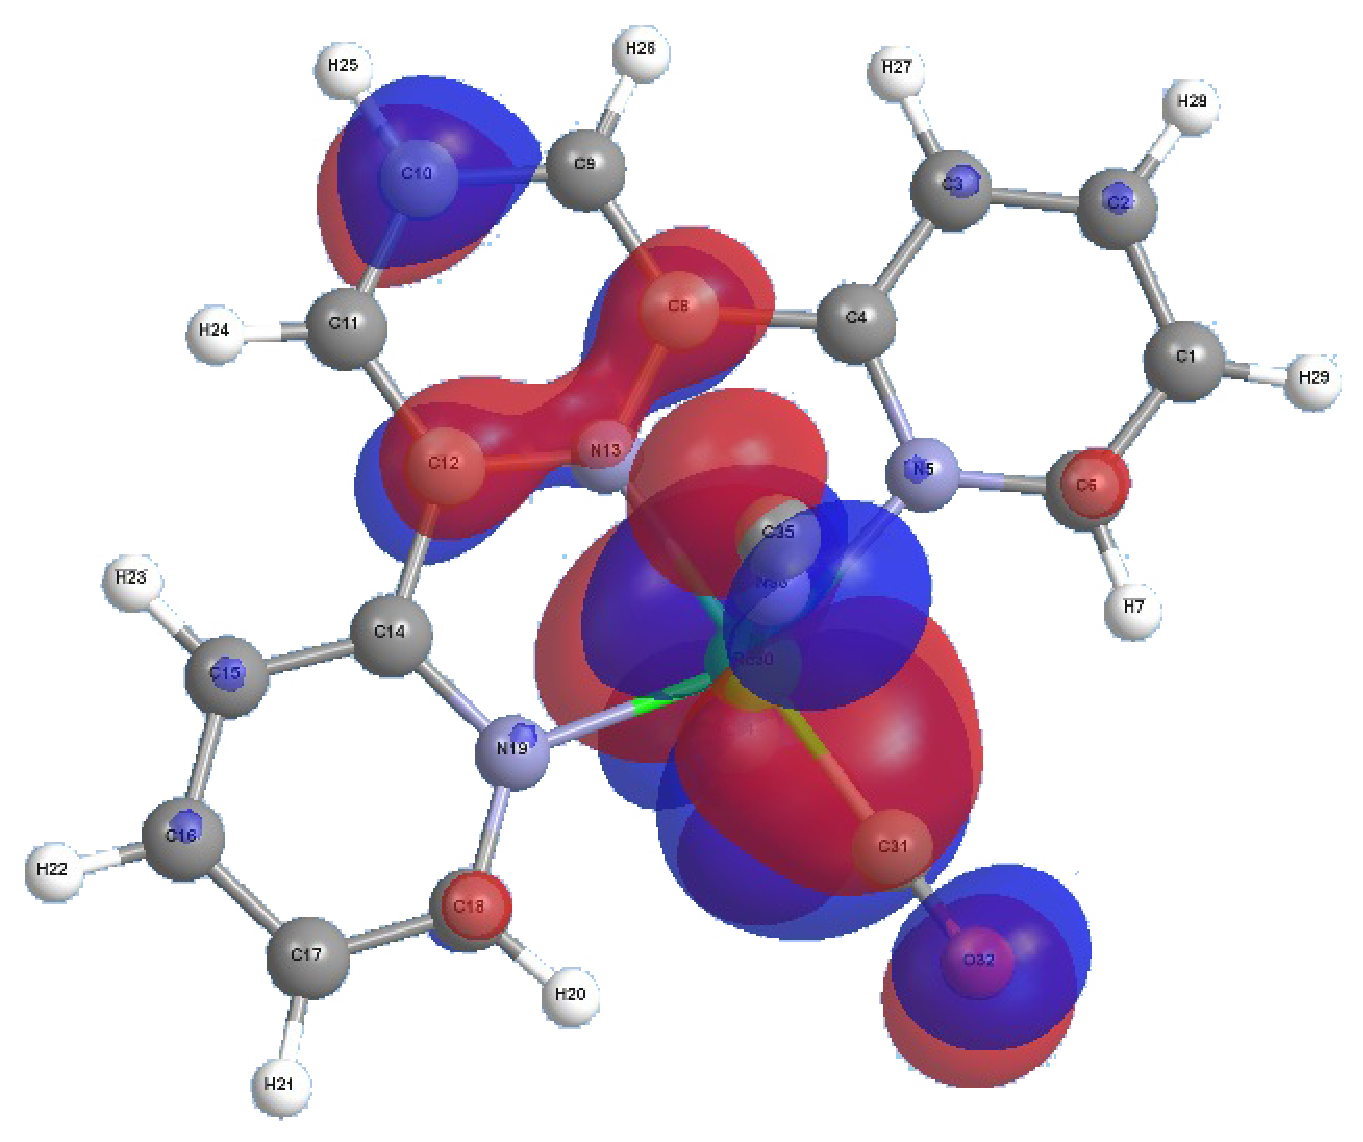
\includegraphics[clip=true, width=\textwidth, keepaspectratio]{images/mos/6h-3.eps}
  \caption{HOMO-3}
 \end{subfigure}
 \begin{subfigure}[b]{0.31\textwidth}
  \includegraphics[clip=true, width=\textwidth, keepaspectratio]{images/mos/6h-4.eps}
  \caption{HOMO-5}
 \end{subfigure}
 \begin{subfigure}[b]{0.31\textwidth}
  \includegraphics[clip=true, width=\textwidth, keepaspectratio]{images/mos/6h-5.eps}
  \caption{HOMO-5}
 \end{subfigure}
\caption[Molecular orbitals HOMO-5 to LUMO+3 of \textbf{2.6}]{Isosurface plots of the frontier molecular orbitals HOMO-5 to LUMO+3 of \textbf{2.6}}
\label{fig.mo26}
\end{figure}

\begin{figure}[!ht]
 \centering
 \begin{subfigure}[b]{0.31\textwidth}
  \includegraphics[clip=true, width=\textwidth, keepaspectratio]{images/mos/7l+2.eps}
  \caption{LUMO+2}
 \end{subfigure}
  \begin{subfigure}[b]{0.31\textwidth}
  \includegraphics[clip=true, width=\textwidth, keepaspectratio]{images/mos/7l+1.eps}
  \caption{LUMO+1}
 \end{subfigure}
  \begin{subfigure}[b]{0.31\textwidth}
  \includegraphics[clip=true, width=\textwidth, keepaspectratio]{images/mos/7l.eps}
  \caption{LUMO}
 \end{subfigure}
 \begin{subfigure}[b]{0.31\textwidth}
  \includegraphics[clip=true, width=\textwidth, keepaspectratio]{images/mos/7h.eps}
  \caption{HOMO}
 \end{subfigure}
 \begin{subfigure}[b]{0.31\textwidth}
  \includegraphics[clip=true, width=\textwidth, keepaspectratio]{images/mos/7h-1.eps}
  \caption{HOMO-1}
 \end{subfigure}
 \begin{subfigure}[b]{0.31\textwidth}
  \includegraphics[clip=true, width=\textwidth, keepaspectratio]{images/mos/7h-2.eps}
  \caption{HOMO-2}
 \end{subfigure}
 \begin{subfigure}[b]{0.31\textwidth}
  \includegraphics[clip=true, width=\textwidth, keepaspectratio]{images/mos/7h-3.eps}
  \caption{HOMO-3}
 \end{subfigure}
\caption[Molecular orbitals HOMO-3 to LUMO+2 of \textbf{2.7}]{Isosurface plots of the frontier molecular orbitals HOMO-3 to LUMO+2 of \textbf{2.7}}
\label{fig.mo27}
\end{figure} 

\begin{figure}[!ht]
 \centering
 \begin{subfigure}[b]{0.31\textwidth}
  \includegraphics[clip=true, width=\textwidth, keepaspectratio]{images/mos/8l+3.eps}
  \caption{LUMO+3}
 \end{subfigure}
 \begin{subfigure}[b]{0.31\textwidth}
  \includegraphics[clip=true, width=\textwidth, keepaspectratio]{images/mos/8l+2.eps}
  \caption{LUMO+2}
 \end{subfigure}
  \begin{subfigure}[b]{0.31\textwidth}
  \includegraphics[clip=true, width=\textwidth, keepaspectratio]{images/mos/8l+1.eps}
  \caption{LUMO+1}
 \end{subfigure}
  \begin{subfigure}[b]{0.31\textwidth}
  \includegraphics[clip=true, width=\textwidth, keepaspectratio]{images/mos/8l.eps}
  \caption{LUMO}
 \end{subfigure}
 \begin{subfigure}[b]{0.31\textwidth}
  \includegraphics[clip=true, width=\textwidth, keepaspectratio]{images/mos/8h.eps}
  \caption{HOMO}
 \end{subfigure}
 \begin{subfigure}[b]{0.31\textwidth}
  \includegraphics[clip=true, width=\textwidth, keepaspectratio]{images/mos/8h-1.eps}
  \caption{HOMO-1}
 \end{subfigure}
 \begin{subfigure}[b]{0.31\textwidth}
  \includegraphics[clip=true, width=\textwidth, keepaspectratio]{images/mos/8h-2.eps}
  \caption{HOMO-2}
 \end{subfigure}
 \begin{subfigure}[b]{0.31\textwidth}
  \includegraphics[clip=true, width=\textwidth, keepaspectratio]{images/mos/8h-3.eps}
  \caption{HOMO-3}
 \end{subfigure}
 \begin{subfigure}[b]{0.31\textwidth}
  \includegraphics[clip=true, width=\textwidth, keepaspectratio]{images/mos/8h-4.eps}
  \caption{HOMO-5}
 \end{subfigure}
 \begin{subfigure}[b]{0.31\textwidth}
  \includegraphics[clip=true, width=\textwidth, keepaspectratio]{images/mos/8h-5.eps}
  \caption{HOMO-5}
 \end{subfigure}
\caption[Molecular orbitals HOMO-5 to LUMO+3 of \textbf{2.8}]{Isosurface plots of the frontier molecular orbitals HOMO-5 to LUMO+3 of \textbf{2.8}}
\label{fig.mo28}
\end{figure}
